\documentclass[1p]{elsarticle_modified}
%\bibliographystyle{elsarticle-num}

%\usepackage[colorlinks]{hyperref}
%\usepackage{abbrmath_seonhwa} %\Abb, \Ascr, \Acal ,\Abf, \Afrak
\usepackage{amsfonts}
\usepackage{amssymb}
\usepackage{amsmath}
\usepackage{amsthm}
\usepackage{scalefnt}
\usepackage{amsbsy}
\usepackage{kotex}
\usepackage{caption}
\usepackage{subfig}
\usepackage{color}
\usepackage{graphicx}
\usepackage{xcolor} %% white, black, red, green, blue, cyan, magenta, yellow
\usepackage{float}
\usepackage{setspace}
\usepackage{hyperref}

\usepackage{tikz}
\usetikzlibrary{arrows}

\usepackage{multirow}
\usepackage{array} % fixed length table
\usepackage{hhline}

%%%%%%%%%%%%%%%%%%%%%
\makeatletter
\renewcommand*\env@matrix[1][\arraystretch]{%
	\edef\arraystretch{#1}%
	\hskip -\arraycolsep
	\let\@ifnextchar\new@ifnextchar
	\array{*\c@MaxMatrixCols c}}
\makeatother %https://tex.stackexchange.com/questions/14071/how-can-i-increase-the-line-spacing-in-a-matrix
%%%%%%%%%%%%%%%

\usepackage[normalem]{ulem}

\newcommand{\msout}[1]{\ifmmode\text{\sout{\ensuremath{#1}}}\else\sout{#1}\fi}
%SOURCE: \msout is \stkout macro in https://tex.stackexchange.com/questions/20609/strikeout-in-math-mode

\newcommand{\cancel}[1]{
	\ifmmode
	{\color{red}\msout{#1}}
	\else
	{\color{red}\sout{#1}}
	\fi
}

\newcommand{\add}[1]{
	{\color{blue}\uwave{#1}}
}

\newcommand{\replace}[2]{
	\ifmmode
	{\color{red}\msout{#1}}{\color{blue}\uwave{#2}}
	\else
	{\color{red}\sout{#1}}{\color{blue}\uwave{#2}}
	\fi
}

\newcommand{\Sol}{\mathcal{S}} %segment
\newcommand{\D}{D} %diagram
\newcommand{\A}{\mathcal{A}} %arc


%%%%%%%%%%%%%%%%%%%%%%%%%%%%%5 test

\def\sl{\operatorname{\textup{SL}}(2,\Cbb)}
\def\psl{\operatorname{\textup{PSL}}(2,\Cbb)}
\def\quan{\mkern 1mu \triangleright \mkern 1mu}

\theoremstyle{definition}
\newtheorem{thm}{Theorem}[section]
\newtheorem{prop}[thm]{Proposition}
\newtheorem{lem}[thm]{Lemma}
\newtheorem{ques}[thm]{Question}
\newtheorem{cor}[thm]{Corollary}
\newtheorem{defn}[thm]{Definition}
\newtheorem{exam}[thm]{Example}
\newtheorem{rmk}[thm]{Remark}
\newtheorem{alg}[thm]{Algorithm}

\newcommand{\I}{\sqrt{-1}}
\begin{document}

%\begin{frontmatter}
%
%\title{Boundary parabolic representations of knots up to 8 crossings}
%
%%% Group authors per affiliation:
%\author{Yunhi Cho} 
%\address{Department of Mathematics, University of Seoul, Seoul, Korea}
%\ead{yhcho@uos.ac.kr}
%
%
%\author{Seonhwa Kim} %\fnref{s_kim}}
%\address{Center for Geometry and Physics, Institute for Basic Science, Pohang, 37673, Korea}
%\ead{ryeona17@ibs.re.kr}
%
%\author{Hyuk Kim}
%\address{Department of Mathematical Sciences, Seoul National University, Seoul 08826, Korea}
%\ead{hyukkim@snu.ac.kr}
%
%\author{Seokbeom Yoon}
%\address{Department of Mathematical Sciences, Seoul National University, Seoul, 08826,  Korea}
%\ead{sbyoon15@snu.ac.kr}
%
%\begin{abstract}
%We find all boundary parabolic representation of knots up to 8 crossings.
%
%\end{abstract}
%\begin{keyword}
%    \MSC[2010] 57M25 
%\end{keyword}
%
%\end{frontmatter}

%\linenumbers
%\tableofcontents
%
\newcommand\colored[1]{\textcolor{white}{\rule[-0.35ex]{0.8em}{1.4ex}}\kern-0.8em\color{red} #1}%
%\newcommand\colored[1]{\textcolor{white}{ #1}\kern-2.17ex	\textcolor{white}{ #1}\kern-1.81ex	\textcolor{white}{ #1}\kern-2.15ex\color{red}#1	}

{\Large $\underline{12a_{0029}~(K12a_{0029})}$}

\setlength{\tabcolsep}{10pt}
\renewcommand{\arraystretch}{1.6}
\vspace{1cm}\begin{tabular}{m{100pt}>{\centering\arraybackslash}m{274pt}}
\multirow{5}{120pt}{
	\centering
	\includegraphics[width=112pt]{../../../GIT/diagram.site/Diagrams/png/830_12a_0029.png}\\
\ \ \ A knot diagram\footnotemark}&
\allowdisplaybreaks
\textbf{Linearized knot diagam} \\
\cline{2-2}
 &
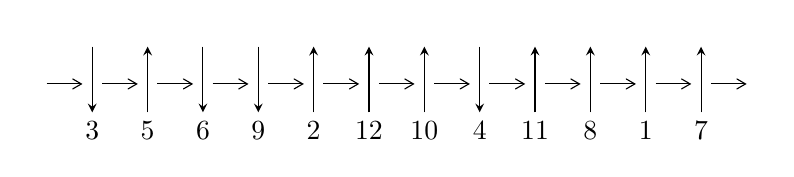
\begin{tikzpicture}[x=20pt, y=17pt]
	% nodes
	\node (C0) at (0, 0) {};
	\node (C1) at (1, 0) {};
	\node (C1U) at (1, +1) {};
	\node (C1D) at (1, -1) {3};

	\node (C2) at (2, 0) {};
	\node (C2U) at (2, +1) {};
	\node (C2D) at (2, -1) {5};

	\node (C3) at (3, 0) {};
	\node (C3U) at (3, +1) {};
	\node (C3D) at (3, -1) {6};

	\node (C4) at (4, 0) {};
	\node (C4U) at (4, +1) {};
	\node (C4D) at (4, -1) {9};

	\node (C5) at (5, 0) {};
	\node (C5U) at (5, +1) {};
	\node (C5D) at (5, -1) {2};

	\node (C6) at (6, 0) {};
	\node (C6U) at (6, +1) {};
	\node (C6D) at (6, -1) {12};

	\node (C7) at (7, 0) {};
	\node (C7U) at (7, +1) {};
	\node (C7D) at (7, -1) {10};

	\node (C8) at (8, 0) {};
	\node (C8U) at (8, +1) {};
	\node (C8D) at (8, -1) {4};

	\node (C9) at (9, 0) {};
	\node (C9U) at (9, +1) {};
	\node (C9D) at (9, -1) {11};

	\node (C10) at (10, 0) {};
	\node (C10U) at (10, +1) {};
	\node (C10D) at (10, -1) {8};

	\node (C11) at (11, 0) {};
	\node (C11U) at (11, +1) {};
	\node (C11D) at (11, -1) {1};

	\node (C12) at (12, 0) {};
	\node (C12U) at (12, +1) {};
	\node (C12D) at (12, -1) {7};
	\node (C13) at (13, 0) {};

	% arrows
	\draw[->,>={angle 60}]
	(C0) edge (C1) (C1) edge (C2) (C2) edge (C3) (C3) edge (C4) (C4) edge (C5) (C5) edge (C6) (C6) edge (C7) (C7) edge (C8) (C8) edge (C9) (C9) edge (C10) (C10) edge (C11) (C11) edge (C12) (C12) edge (C13) ;	\draw[->,>=stealth]
	(C1U) edge (C1D) (C2D) edge (C2U) (C3U) edge (C3D) (C4U) edge (C4D) (C5D) edge (C5U) (C6D) edge (C6U) (C7D) edge (C7U) (C8U) edge (C8D) (C9D) edge (C9U) (C10D) edge (C10U) (C11D) edge (C11U) (C12D) edge (C12U) ;
	\end{tikzpicture} \\
\hhline{~~} \\& 
\textbf{Solving Sequence} \\ \cline{2-2} 
 &
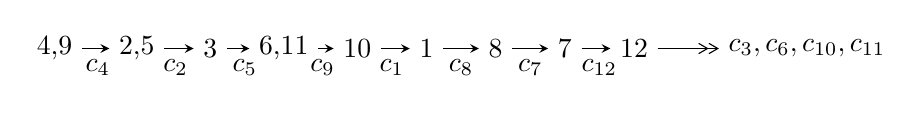
\begin{tikzpicture}[x=25pt, y=7pt]
	% node
	\node (A0) at (-1/8, 0) {4,9};
	\node (A1) at (17/16, 0) {2,5};
	\node (A2) at (17/8, 0) {3};
	\node (A3) at (51/16, 0) {6,11};
	\node (A4) at (17/4, 0) {10};
	\node (A5) at (21/4, 0) {1};
	\node (A6) at (25/4, 0) {8};
	\node (A7) at (29/4, 0) {7};
	\node (A8) at (33/4, 0) {12};
	\node (C1) at (1/2, -1) {$c_{4}$};
	\node (C2) at (13/8, -1) {$c_{2}$};
	\node (C3) at (21/8, -1) {$c_{5}$};
	\node (C4) at (15/4, -1) {$c_{9}$};
	\node (C5) at (19/4, -1) {$c_{1}$};
	\node (C6) at (23/4, -1) {$c_{8}$};
	\node (C7) at (27/4, -1) {$c_{7}$};
	\node (C8) at (31/4, -1) {$c_{12}$};
	\node (A9) at (43/4, 0) {$c_{3},c_{6},c_{10},c_{11}$};

	% edge
	\draw[->,>=stealth]	
	(A0) edge (A1) (A1) edge (A2) (A2) edge (A3) (A3) edge (A4) (A4) edge (A5) (A5) edge (A6) (A6) edge (A7) (A7) edge (A8) ;
	\draw[->>,>={angle 60}]	
	(A8) edge (A9);
\end{tikzpicture} \\ 

\end{tabular} \\

\footnotetext{
The image of knot diagram is generated by the software ``\textbf{Draw programme}" developed by Andrew Bartholomew(\url{http://www.layer8.co.uk/maths/draw/index.htm\#Running-draw}), where we modified some parts for our purpose(\url{https://github.com/CATsTAILs/LinksPainter}).
}\phantom \\ \newline 
\centering \textbf{Ideals for irreducible components\footnotemark of $X_{\text{par}}$} 
 
\begin{align*}
I^u_{1}&=\langle 
4.48200\times10^{61} u^{45}-9.22155\times10^{61} u^{44}+\cdots+1.04756\times10^{63} d-1.67459\times10^{63},\\
\phantom{I^u_{1}}&\phantom{= \langle  }7.62250\times10^{61} u^{45}-1.89258\times10^{62} u^{44}+\cdots+2.09512\times10^{63} c-3.36115\times10^{63},\\
\phantom{I^u_{1}}&\phantom{= \langle  }1.37141\times10^{61} u^{45}-2.04563\times10^{61} u^{44}+\cdots+1.04756\times10^{63} b-1.27647\times10^{63},\\
\phantom{I^u_{1}}&\phantom{= \langle  }7.65358\times10^{61} u^{45}-2.24209\times10^{62} u^{44}+\cdots+1.04756\times10^{63} a-1.33042\times10^{62},\;u^{46}-3 u^{45}+\cdots-32 u+32\rangle \\
I^u_{2}&=\langle 
-5.05017\times10^{19} c u^{37}+2.57220\times10^{19} u^{37}+\cdots+1.77366\times10^{20} c+1.40518\times10^{20},\\
\phantom{I^u_{2}}&\phantom{= \langle  }-1.48141\times10^{20} c u^{37}+8.78585\times10^{19} u^{37}+\cdots+1.69449\times10^{19} c-1.02888\times10^{20},\\
\phantom{I^u_{2}}&\phantom{= \langle  }-3.80860\times10^{20} u^{37}-1.22578\times10^{20} u^{36}+\cdots+3.70123\times10^{20} b+1.73663\times10^{21},\\
\phantom{I^u_{2}}&\phantom{= \langle  }-9.01587\times10^{20} u^{37}-1.40080\times10^{20} u^{36}+\cdots+7.40247\times10^{20} a+2.56553\times10^{21},\;u^{38}+u^{37}+\cdots+4 u-4\rangle \\
\\
I^v_{1}&=\langle 
a,\;d,\;c- v,\;b- v,\;v^2- v+1\rangle \\
I^v_{2}&=\langle 
a,\;d- v+1,\;- a v+c+1,\;b- v,\;v^2- v+1\rangle \\
I^v_{3}&=\langle 
c,\;d-1,\;b,\;a-1,\;v+1\rangle \\
I^v_{4}&=\langle 
a,\;d b+d a- c b- d+b-1,\;a^2 d- c b a- d a+c b+b a+d- c- a+1,\;d v+1,\;c v- b a- b v+b+a,\\
\phantom{I^v_{4}}&\phantom{= \langle  }b^2- b+1\rangle \\
\end{align*}
\raggedright * 5 irreducible components of $\dim_{\mathbb{C}}=0$, with total 127 representations.\\
\raggedright * 1 irreducible components of $\dim_{\mathbb{C}}=1$ \\
\footnotetext{All coefficients of polynomials are rational numbers. But the coefficients are sometimes approximated in decimal forms when there is not enough margin.}
\newpage
\renewcommand{\arraystretch}{1}
\centering \section*{I. $I^u_{1}= \langle 4.48\times10^{61} u^{45}-9.22\times10^{61} u^{44}+\cdots+1.05\times10^{63} d-1.67\times10^{63},\;7.62\times10^{61} u^{45}-1.89\times10^{62} u^{44}+\cdots+2.10\times10^{63} c-3.36\times10^{63},\;1.37\times10^{61} u^{45}-2.05\times10^{61} u^{44}+\cdots+1.05\times10^{63} b-1.28\times10^{63},\;7.65\times10^{61} u^{45}-2.24\times10^{62} u^{44}+\cdots+1.05\times10^{63} a-1.33\times10^{62},\;u^{46}-3 u^{45}+\cdots-32 u+32 \rangle$}
\flushleft \textbf{(i) Arc colorings}\\
\begin{tabular}{m{7pt} m{180pt} m{7pt} m{180pt} }
\flushright $a_{4}=$&$\begin{pmatrix}1\\0\end{pmatrix}$ \\
\flushright $a_{9}=$&$\begin{pmatrix}0\\u\end{pmatrix}$ \\
\flushright $a_{2}=$&$\begin{pmatrix}-0.0730608 u^{45}+0.214029 u^{44}+\cdots-11.1865 u+0.127001\\-0.0130915 u^{45}+0.0195275 u^{44}+\cdots+0.982266 u+1.21851\end{pmatrix}$ \\
\flushright $a_{5}=$&$\begin{pmatrix}1\\u^2\end{pmatrix}$ \\
\flushright $a_{3}=$&$\begin{pmatrix}-0.107506 u^{45}+0.286640 u^{44}+\cdots-12.3773 u+1.18060\\-0.0329822 u^{45}+0.0562768 u^{44}+\cdots+1.10132 u+2.20169\end{pmatrix}$ \\
\flushright $a_{6}=$&$\begin{pmatrix}-0.0337179 u^{45}+0.143074 u^{44}+\cdots-8.46741 u+4.71002\\0.0470900 u^{45}-0.103838 u^{44}+\cdots+1.16123 u-2.01452\end{pmatrix}$ \\
\flushright $a_{11}=$&$\begin{pmatrix}-0.0363821 u^{45}+0.0903327 u^{44}+\cdots-1.88200 u+1.60427\\-0.0427850 u^{45}+0.0880286 u^{44}+\cdots+0.686956 u+1.59856\end{pmatrix}$ \\
\flushright $a_{10}=$&$\begin{pmatrix}-0.0168951 u^{45}+0.0465535 u^{44}+\cdots-1.39848 u+0.915857\\-0.0232980 u^{45}+0.0442495 u^{44}+\cdots+1.17047 u+0.910145\end{pmatrix}$ \\
\flushright $a_{1}=$&$\begin{pmatrix}-0.0808079 u^{45}+0.246912 u^{44}+\cdots-9.62863 u+6.72455\\-0.0570466 u^{45}+0.0968746 u^{44}+\cdots+1.56827 u+1.87088\end{pmatrix}$ \\
\flushright $a_{8}=$&$\begin{pmatrix}u\\u\end{pmatrix}$ \\
\flushright $a_{7}=$&$\begin{pmatrix}0.00655998 u^{45}-0.0259377 u^{44}+\cdots+2.00677 u-0.607746\\-0.0298221 u^{45}+0.0643950 u^{44}+\cdots+0.124764 u+0.996524\end{pmatrix}$ \\
\flushright $a_{12}=$&$\begin{pmatrix}-0.0639128 u^{45}+0.200359 u^{44}+\cdots-8.23015 u+5.80869\\-0.0337486 u^{45}+0.0526252 u^{44}+\cdots+1.39779 u+0.960739\end{pmatrix}$\\&\end{tabular}
\flushleft \textbf{(ii) Obstruction class $= -1$}\\~\\
\flushleft \textbf{(iii) Cusp Shapes $= 0.247381 u^{45}-0.445802 u^{44}+\cdots-4.44172 u-0.790830$}\\~\\
\newpage\renewcommand{\arraystretch}{1}
\flushleft \textbf{(iv) u-Polynomials at the component}\newline \\
\begin{tabular}{m{50pt}|m{274pt}}
Crossings & \hspace{64pt}u-Polynomials at each crossing \\
\hline $$\begin{aligned}c_{1}\end{aligned}$$&$\begin{aligned}
&u^{46}+21 u^{45}+\cdots-40 u+16
\end{aligned}$\\
\hline $$\begin{aligned}c_{2},c_{5}\end{aligned}$$&$\begin{aligned}
&u^{46}+u^{45}+\cdots-4 u+4
\end{aligned}$\\
\hline $$\begin{aligned}c_{3}\end{aligned}$$&$\begin{aligned}
&u^{46}- u^{45}+\cdots-2596 u+1252
\end{aligned}$\\
\hline $$\begin{aligned}c_{4},c_{8}\end{aligned}$$&$\begin{aligned}
&u^{46}-3 u^{45}+\cdots-32 u+32
\end{aligned}$\\
\hline $$\begin{aligned}c_{6},c_{7},c_{10}\\c_{12}\end{aligned}$$&$\begin{aligned}
&u^{46}+5 u^{45}+\cdots+2 u+1
\end{aligned}$\\
\hline $$\begin{aligned}c_{9},c_{11}\end{aligned}$$&$\begin{aligned}
&u^{46}-21 u^{45}+\cdots+4 u+1
\end{aligned}$\\
\hline
\end{tabular}\\~\\
\newpage\renewcommand{\arraystretch}{1}
\flushleft \textbf{(v) Riley Polynomials at the component}\newline \\
\begin{tabular}{m{50pt}|m{274pt}}
Crossings & \hspace{64pt}Riley Polynomials at each crossing \\
\hline $$\begin{aligned}c_{1}\end{aligned}$$&$\begin{aligned}
&y^{46}+9 y^{45}+\cdots-5664 y+256
\end{aligned}$\\
\hline $$\begin{aligned}c_{2},c_{5}\end{aligned}$$&$\begin{aligned}
&y^{46}+21 y^{45}+\cdots-40 y+16
\end{aligned}$\\
\hline $$\begin{aligned}c_{3}\end{aligned}$$&$\begin{aligned}
&y^{46}-3 y^{45}+\cdots-20408552 y+1567504
\end{aligned}$\\
\hline $$\begin{aligned}c_{4},c_{8}\end{aligned}$$&$\begin{aligned}
&y^{46}-15 y^{45}+\cdots+4096 y+1024
\end{aligned}$\\
\hline $$\begin{aligned}c_{6},c_{7},c_{10}\\c_{12}\end{aligned}$$&$\begin{aligned}
&y^{46}-21 y^{45}+\cdots+4 y+1
\end{aligned}$\\
\hline $$\begin{aligned}c_{9},c_{11}\end{aligned}$$&$\begin{aligned}
&y^{46}+19 y^{45}+\cdots-72 y+1
\end{aligned}$\\
\hline
\end{tabular}\\~\\
\newpage\flushleft \textbf{(vi) Complex Volumes and Cusp Shapes}
$$\begin{array}{c|c|c}  
\text{Solutions to }I^u_{1}& \I (\text{vol} + \sqrt{-1}CS) & \text{Cusp shape}\\
 \hline 
\begin{aligned}
u &= \phantom{-}0.248116 + 0.949341 I \\
a &= \phantom{-}0.659883 - 0.533852 I \\
b &= \phantom{-}0.16697 + 1.82340 I \\
c &= -0.570373 + 0.029986 I \\
d &= -0.088362 + 0.621385 I\end{aligned}
 & -1.66114 + 2.12776 I & -0.422256 - 0.234121 I \\ \hline\begin{aligned}
u &= \phantom{-}0.248116 - 0.949341 I \\
a &= \phantom{-}0.659883 + 0.533852 I \\
b &= \phantom{-}0.16697 - 1.82340 I \\
c &= -0.570373 - 0.029986 I \\
d &= -0.088362 - 0.621385 I\end{aligned}
 & -1.66114 - 2.12776 I & -0.422256 + 0.234121 I \\ \hline\begin{aligned}
u &= -0.642875 + 0.814816 I \\
a &= \phantom{-}0.006254 + 1.275600 I \\
b &= \phantom{-}0.634122 + 0.252731 I \\
c &= -1.335160 - 0.293800 I \\
d &= -0.362590 + 0.315550 I\end{aligned}
 & \phantom{-}5.93091 - 3.99675 I & \phantom{-}10.51051 + 4.44974 I \\ \hline\begin{aligned}
u &= -0.642875 - 0.814816 I \\
a &= \phantom{-}0.006254 - 1.275600 I \\
b &= \phantom{-}0.634122 - 0.252731 I \\
c &= -1.335160 + 0.293800 I \\
d &= -0.362590 - 0.315550 I\end{aligned}
 & \phantom{-}5.93091 + 3.99675 I & \phantom{-}10.51051 - 4.44974 I \\ \hline\begin{aligned}
u &= -0.046642 + 1.050320 I \\
a &= \phantom{-}0.666501 + 0.584237 I \\
b &= -0.27294 - 1.79729 I \\
c &= -0.807442 - 0.110962 I \\
d &= -0.214208 + 0.539648 I\end{aligned}
 & -2.04690 - 4.94372 I & \phantom{-}0.16550 + 7.58166 I \\ \hline\begin{aligned}
u &= -0.046642 - 1.050320 I \\
a &= \phantom{-}0.666501 - 0.584237 I \\
b &= -0.27294 + 1.79729 I \\
c &= -0.807442 + 0.110962 I \\
d &= -0.214208 - 0.539648 I\end{aligned}
 & -2.04690 + 4.94372 I & \phantom{-}0.16550 - 7.58166 I\\
 \hline 
 \end{array}$$\newpage$$\begin{array}{c|c|c}  
\text{Solutions to }I^u_{1}& \I (\text{vol} + \sqrt{-1}CS) & \text{Cusp shape}\\
 \hline 
\begin{aligned}
u &= \phantom{-}0.614432 + 0.696436 I \\
a &= -3.11307 - 1.54198 I \\
b &= \phantom{-}1.05080 - 1.50344 I \\
c &= \phantom{-}1.39259 - 0.38277 I \\
d &= \phantom{-}0.334763 + 0.277573 I\end{aligned}
 & \phantom{-}4.70063 - 1.01560 I & \phantom{-}8.78023 + 1.30126 I \\ \hline\begin{aligned}
u &= \phantom{-}0.614432 - 0.696436 I \\
a &= -3.11307 + 1.54198 I \\
b &= \phantom{-}1.05080 + 1.50344 I \\
c &= \phantom{-}1.39259 + 0.38277 I \\
d &= \phantom{-}0.334763 - 0.277573 I\end{aligned}
 & \phantom{-}4.70063 + 1.01560 I & \phantom{-}8.78023 - 1.30126 I \\ \hline\begin{aligned}
u &= \phantom{-}0.904459 + 0.035006 I \\
a &= \phantom{-}0.684510 + 0.349167 I \\
b &= \phantom{-}1.217210 - 0.498628 I \\
c &= \phantom{-}0.226719 - 0.709857 I \\
d &= \phantom{-}0.94895 - 1.25909 I\end{aligned}
 & \phantom{-}0.23417 - 4.06154 I & \phantom{-}0.42563 + 7.90074 I \\ \hline\begin{aligned}
u &= \phantom{-}0.904459 - 0.035006 I \\
a &= \phantom{-}0.684510 - 0.349167 I \\
b &= \phantom{-}1.217210 + 0.498628 I \\
c &= \phantom{-}0.226719 + 0.709857 I \\
d &= \phantom{-}0.94895 + 1.25909 I\end{aligned}
 & \phantom{-}0.23417 + 4.06154 I & \phantom{-}0.42563 - 7.90074 I \\ \hline\begin{aligned}
u &= \phantom{-}0.517103 + 1.038360 I \\
a &= \phantom{-}0.728606 + 0.786743 I \\
b &= -1.25298 - 0.96152 I \\
c &= \phantom{-}1.178790 - 0.188129 I \\
d &= \phantom{-}0.361203 + 0.412386 I\end{aligned}
 & \phantom{-}0.12548 + 4.11136 I & \phantom{-}2.46017 - 3.87123 I \\ \hline\begin{aligned}
u &= \phantom{-}0.517103 - 1.038360 I \\
a &= \phantom{-}0.728606 - 0.786743 I \\
b &= -1.25298 + 0.96152 I \\
c &= \phantom{-}1.178790 + 0.188129 I \\
d &= \phantom{-}0.361203 - 0.412386 I\end{aligned}
 & \phantom{-}0.12548 - 4.11136 I & \phantom{-}2.46017 + 3.87123 I\\
 \hline 
 \end{array}$$\newpage$$\begin{array}{c|c|c}  
\text{Solutions to }I^u_{1}& \I (\text{vol} + \sqrt{-1}CS) & \text{Cusp shape}\\
 \hline 
\begin{aligned}
u &= \phantom{-}0.017678 + 0.820472 I \\
a &= \phantom{-}0.853788 + 0.005623 I \\
b &= -0.0664210 + 0.0072212 I \\
c &= \phantom{-}0.617736 - 0.298148 I \\
d &= \phantom{-}0.123361 + 0.470883 I\end{aligned}
 & \phantom{-}0.79101 + 1.46703 I & \phantom{-}5.32252 - 4.75359 I \\ \hline\begin{aligned}
u &= \phantom{-}0.017678 - 0.820472 I \\
a &= \phantom{-}0.853788 - 0.005623 I \\
b &= -0.0664210 - 0.0072212 I \\
c &= \phantom{-}0.617736 + 0.298148 I \\
d &= \phantom{-}0.123361 - 0.470883 I\end{aligned}
 & \phantom{-}0.79101 - 1.46703 I & \phantom{-}5.32252 + 4.75359 I \\ \hline\begin{aligned}
u &= \phantom{-}1.006520 + 0.624064 I \\
a &= \phantom{-}0.618102 - 0.412984 I \\
b &= \phantom{-}1.58573 + 1.52879 I \\
c &= \phantom{-}0.186343 - 1.252860 I \\
d &= \phantom{-}0.75459 - 2.11694 I\end{aligned}
 & \phantom{-}3.52144 - 4.08819 I & \phantom{-}5.82465 + 4.54278 I \\ \hline\begin{aligned}
u &= \phantom{-}1.006520 - 0.624064 I \\
a &= \phantom{-}0.618102 + 0.412984 I \\
b &= \phantom{-}1.58573 - 1.52879 I \\
c &= \phantom{-}0.186343 + 1.252860 I \\
d &= \phantom{-}0.75459 + 2.11694 I\end{aligned}
 & \phantom{-}3.52144 + 4.08819 I & \phantom{-}5.82465 - 4.54278 I \\ \hline\begin{aligned}
u &= -1.071740 + 0.508840 I \\
a &= \phantom{-}0.249412 + 0.451516 I \\
b &= -0.037567 + 0.421763 I \\
c &= \phantom{-}0.237093 + 0.582132 I \\
d &= -0.291926 + 1.082080 I\end{aligned}
 & -1.98761 + 2.55534 I & \phantom{-}0.98949 - 1.01939 I \\ \hline\begin{aligned}
u &= -1.071740 - 0.508840 I \\
a &= \phantom{-}0.249412 - 0.451516 I \\
b &= -0.037567 - 0.421763 I \\
c &= \phantom{-}0.237093 - 0.582132 I \\
d &= -0.291926 - 1.082080 I\end{aligned}
 & -1.98761 - 2.55534 I & \phantom{-}0.98949 + 1.01939 I\\
 \hline 
 \end{array}$$\newpage$$\begin{array}{c|c|c}  
\text{Solutions to }I^u_{1}& \I (\text{vol} + \sqrt{-1}CS) & \text{Cusp shape}\\
 \hline 
\begin{aligned}
u &= -0.807683 + 0.082878 I \\
a &= \phantom{-}0.701991 - 0.351361 I \\
b &= \phantom{-}1.056930 + 0.488868 I \\
c &= -0.192599 + 0.514963 I \\
d &= -0.891839 + 0.948808 I\end{aligned}
 & \phantom{-}0.274017 + 1.087600 I & -0.651009 + 0.594713 I \\ \hline\begin{aligned}
u &= -0.807683 - 0.082878 I \\
a &= \phantom{-}0.701991 + 0.351361 I \\
b &= \phantom{-}1.056930 - 0.488868 I \\
c &= -0.192599 - 0.514963 I \\
d &= -0.891839 - 0.948808 I\end{aligned}
 & \phantom{-}0.274017 - 1.087600 I & -0.651009 - 0.594713 I \\ \hline\begin{aligned}
u &= -0.668777 + 1.013930 I \\
a &= \phantom{-}0.733154 - 0.148233 I \\
b &= \phantom{-}0.143797 - 0.527077 I \\
c &= -1.276030 - 0.170948 I \\
d &= -0.403997 + 0.376312 I\end{aligned}
 & \phantom{-}4.90536 - 6.51831 I & \phantom{-}8.90536 + 4.64881 I \\ \hline\begin{aligned}
u &= -0.668777 - 1.013930 I \\
a &= \phantom{-}0.733154 + 0.148233 I \\
b &= \phantom{-}0.143797 + 0.527077 I \\
c &= -1.276030 + 0.170948 I \\
d &= -0.403997 - 0.376312 I\end{aligned}
 & \phantom{-}4.90536 + 6.51831 I & \phantom{-}8.90536 - 4.64881 I \\ \hline\begin{aligned}
u &= -1.035500 + 0.682470 I \\
a &= \phantom{-}0.691378 - 0.235874 I \\
b &= \phantom{-}0.882817 - 0.508436 I \\
c &= -0.156215 - 1.277950 I \\
d &= -0.69298 - 2.14399 I\end{aligned}
 & \phantom{-}4.70874 + 9.62616 I & \phantom{-}7.79470 - 8.99124 I \\ \hline\begin{aligned}
u &= -1.035500 - 0.682470 I \\
a &= \phantom{-}0.691378 + 0.235874 I \\
b &= \phantom{-}0.882817 + 0.508436 I \\
c &= -0.156215 + 1.277950 I \\
d &= -0.69298 + 2.14399 I\end{aligned}
 & \phantom{-}4.70874 - 9.62616 I & \phantom{-}7.79470 + 8.99124 I\\
 \hline 
 \end{array}$$\newpage$$\begin{array}{c|c|c}  
\text{Solutions to }I^u_{1}& \I (\text{vol} + \sqrt{-1}CS) & \text{Cusp shape}\\
 \hline 
\begin{aligned}
u &= \phantom{-}1.224990 + 0.226721 I \\
a &= \phantom{-}0.253462 - 0.169367 I \\
b &= -0.320531 - 0.225417 I \\
c &= \phantom{-}0.050461 - 0.989550 I \\
d &= \phantom{-}0.63809 - 1.66040 I\end{aligned}
 & -3.57586 - 5.30392 I & \phantom{-}1.93777 + 5.96454 I \\ \hline\begin{aligned}
u &= \phantom{-}1.224990 - 0.226721 I \\
a &= \phantom{-}0.253462 + 0.169367 I \\
b &= -0.320531 + 0.225417 I \\
c &= \phantom{-}0.050461 + 0.989550 I \\
d &= \phantom{-}0.63809 + 1.66040 I\end{aligned}
 & -3.57586 + 5.30392 I & \phantom{-}1.93777 - 5.96454 I \\ \hline\begin{aligned}
u &= \phantom{-}1.195740 + 0.364671 I \\
a &= \phantom{-}0.44005 + 1.75493 I \\
b &= -1.22042 + 1.50844 I \\
c &= -0.186101 + 0.688056 I \\
d &= \phantom{-}0.356273 + 1.213420 I\end{aligned}
 & -6.39735 + 0.44189 I & -4.43091 - 2.06201 I \\ \hline\begin{aligned}
u &= \phantom{-}1.195740 - 0.364671 I \\
a &= \phantom{-}0.44005 - 1.75493 I \\
b &= -1.22042 - 1.50844 I \\
c &= -0.186101 - 0.688056 I \\
d &= \phantom{-}0.356273 - 1.213420 I\end{aligned}
 & -6.39735 - 0.44189 I & -4.43091 + 2.06201 I \\ \hline\begin{aligned}
u &= \phantom{-}0.687704 + 1.079720 I \\
a &= \phantom{-}0.598930 - 0.485617 I \\
b &= \phantom{-}0.89116 + 2.33948 I \\
c &= \phantom{-}1.270960 - 0.132505 I \\
d &= \phantom{-}0.421173 + 0.392926 I\end{aligned}
 & \phantom{-}2.74057 + 11.63170 I & \phantom{-}5.60201 - 8.64749 I \\ \hline\begin{aligned}
u &= \phantom{-}0.687704 - 1.079720 I \\
a &= \phantom{-}0.598930 + 0.485617 I \\
b &= \phantom{-}0.89116 - 2.33948 I \\
c &= \phantom{-}1.270960 + 0.132505 I \\
d &= \phantom{-}0.421173 - 0.392926 I\end{aligned}
 & \phantom{-}2.74057 - 11.63170 I & \phantom{-}5.60201 + 8.64749 I\\
 \hline 
 \end{array}$$\newpage$$\begin{array}{c|c|c}  
\text{Solutions to }I^u_{1}& \I (\text{vol} + \sqrt{-1}CS) & \text{Cusp shape}\\
 \hline 
\begin{aligned}
u &= \phantom{-}1.158970 + 0.578549 I \\
a &= -1.27784 - 1.84483 I \\
b &= \phantom{-}0.63049 - 2.44257 I \\
c &= -0.292580 + 0.618138 I \\
d &= \phantom{-}0.226552 + 1.126520 I\end{aligned}
 & -4.42926 - 7.47789 I & -1.74286 + 4.84208 I \\ \hline\begin{aligned}
u &= \phantom{-}1.158970 - 0.578549 I \\
a &= -1.27784 + 1.84483 I \\
b &= \phantom{-}0.63049 + 2.44257 I \\
c &= -0.292580 - 0.618138 I \\
d &= \phantom{-}0.226552 - 1.126520 I\end{aligned}
 & -4.42926 + 7.47789 I & -1.74286 - 4.84208 I \\ \hline\begin{aligned}
u &= -1.311140 + 0.102134 I \\
a &= \phantom{-}0.00268 - 1.92087 I \\
b &= -0.86720 - 2.10727 I \\
c &= \phantom{-}0.030662 - 0.940031 I \\
d &= -0.53344 - 1.57008 I\end{aligned}
 & -7.51022 + 1.50301 I & -3.10935 - 2.27720 I \\ \hline\begin{aligned}
u &= -1.311140 - 0.102134 I \\
a &= \phantom{-}0.00268 + 1.92087 I \\
b &= -0.86720 + 2.10727 I \\
c &= \phantom{-}0.030662 + 0.940031 I \\
d &= -0.53344 + 1.57008 I\end{aligned}
 & -7.51022 - 1.50301 I & -3.10935 + 2.27720 I \\ \hline\begin{aligned}
u &= -0.435796 + 0.485308 I \\
a &= \phantom{-}0.873003 - 0.355186 I \\
b &= \phantom{-}0.215705 + 0.325189 I \\
c &= \phantom{-}0.168435 + 0.132484 I \\
d &= -0.223442 + 0.550785 I\end{aligned}
 & -0.084212 + 1.381070 I & -0.30299 - 4.86269 I \\ \hline\begin{aligned}
u &= -0.435796 - 0.485308 I \\
a &= \phantom{-}0.873003 + 0.355186 I \\
b &= \phantom{-}0.215705 - 0.325189 I \\
c &= \phantom{-}0.168435 - 0.132484 I \\
d &= -0.223442 - 0.550785 I\end{aligned}
 & -0.084212 - 1.381070 I & -0.30299 + 4.86269 I\\
 \hline 
 \end{array}$$\newpage$$\begin{array}{c|c|c}  
\text{Solutions to }I^u_{1}& \I (\text{vol} + \sqrt{-1}CS) & \text{Cusp shape}\\
 \hline 
\begin{aligned}
u &= -1.316840 + 0.304432 I \\
a &= -0.68441 + 1.94019 I \\
b &= -0.04666 + 2.56224 I \\
c &= -0.010549 - 1.050770 I \\
d &= -0.56280 - 1.73815 I\end{aligned}
 & -6.69471 + 9.89538 I & -1.12698 - 9.02462 I \\ \hline\begin{aligned}
u &= -1.316840 - 0.304432 I \\
a &= -0.68441 - 1.94019 I \\
b &= -0.04666 - 2.56224 I \\
c &= -0.010549 + 1.050770 I \\
d &= -0.56280 + 1.73815 I\end{aligned}
 & -6.69471 - 9.89538 I & -1.12698 + 9.02462 I \\ \hline\begin{aligned}
u &= -1.118430 + 0.781907 I \\
a &= \phantom{-}0.006550 + 0.558246 I \\
b &= \phantom{-}0.136959 + 0.741041 I \\
c &= -0.096143 - 1.306940 I \\
d &= -0.58055 - 2.15879 I\end{aligned}
 & \phantom{-}3.44989 + 13.07100 I & \phantom{-}7.52581 - 7.90184 I \\ \hline\begin{aligned}
u &= -1.118430 - 0.781907 I \\
a &= \phantom{-}0.006550 - 0.558246 I \\
b &= \phantom{-}0.136959 - 0.741041 I \\
c &= -0.096143 + 1.306940 I \\
d &= -0.58055 + 2.15879 I\end{aligned}
 & \phantom{-}3.44989 - 13.07100 I & \phantom{-}7.52581 + 7.90184 I \\ \hline\begin{aligned}
u &= \phantom{-}1.166960 + 0.709743 I \\
a &= \phantom{-}0.55758 + 1.32715 I \\
b &= -1.85153 + 0.87351 I \\
c &= \phantom{-}0.086648 - 1.266670 I \\
d &= \phantom{-}0.58757 - 2.09046 I\end{aligned}
 & -1.96462 - 10.42030 I & \phantom{-0.000000 -}0. + 7.01224 I \\ \hline\begin{aligned}
u &= \phantom{-}1.166960 - 0.709743 I \\
a &= \phantom{-}0.55758 - 1.32715 I \\
b &= -1.85153 - 0.87351 I \\
c &= \phantom{-}0.086648 + 1.266670 I \\
d &= \phantom{-}0.58757 + 2.09046 I\end{aligned}
 & -1.96462 + 10.42030 I & \phantom{-0.000000 } 0. - 7.01224 I\\
 \hline 
 \end{array}$$\newpage$$\begin{array}{c|c|c}  
\text{Solutions to }I^u_{1}& \I (\text{vol} + \sqrt{-1}CS) & \text{Cusp shape}\\
 \hline 
\begin{aligned}
u &= \phantom{-}1.144720 + 0.813548 I \\
a &= -1.46199 - 1.44274 I \\
b &= \phantom{-}1.12386 - 2.52551 I \\
c &= \phantom{-}0.079457 - 1.315210 I \\
d &= \phantom{-}0.54947 - 2.16215 I\end{aligned}
 & \phantom{-}1.2351 - 18.4885 I & \phantom{-}4.00000 + 11.60486 I \\ \hline\begin{aligned}
u &= \phantom{-}1.144720 - 0.813548 I \\
a &= -1.46199 + 1.44274 I \\
b &= \phantom{-}1.12386 + 2.52551 I \\
c &= \phantom{-}0.079457 + 1.315210 I \\
d &= \phantom{-}0.54947 + 2.16215 I\end{aligned}
 & \phantom{-}1.2351 + 18.4885 I & \phantom{-}4.00000 - 11.60486 I \\ \hline\begin{aligned}
u &= \phantom{-}0.068034 + 0.485475 I \\
a &= -3.28852 - 7.48764 I \\
b &= \phantom{-}0.699694 + 0.686768 I \\
c &= \phantom{-}0.39729 - 1.46311 I \\
d &= \phantom{-}0.044140 + 0.259666 I\end{aligned}
 & \phantom{-}2.91211 + 2.24138 I & \phantom{-}11.31463 - 3.80305 I \\ \hline\begin{aligned}
u &= \phantom{-}0.068034 - 0.485475 I \\
a &= -3.28852 + 7.48764 I \\
b &= \phantom{-}0.699694 - 0.686768 I \\
c &= \phantom{-}0.39729 + 1.46311 I \\
d &= \phantom{-}0.044140 - 0.259666 I\end{aligned}
 & \phantom{-}2.91211 - 2.24138 I & \phantom{-}11.31463 + 3.80305 I\\
 \hline 
 \end{array}$$\newpage\newpage\renewcommand{\arraystretch}{1}
\centering \section*{II. $I^u_{2}= \langle -5.05\times10^{19} c u^{37}+2.57\times10^{19} u^{37}+\cdots+1.77\times10^{20} c+1.41\times10^{20},\;-1.48\times10^{20} c u^{37}+8.79\times10^{19} u^{37}+\cdots+1.69\times10^{19} c-1.03\times10^{20},\;-3.81\times10^{20} u^{37}-1.23\times10^{20} u^{36}+\cdots+3.70\times10^{20} b+1.74\times10^{21},\;-9.02\times10^{20} u^{37}-1.40\times10^{20} u^{36}+\cdots+7.40\times10^{20} a+2.57\times10^{21},\;u^{38}+u^{37}+\cdots+4 u-4 \rangle$}
\flushleft \textbf{(i) Arc colorings}\\
\begin{tabular}{m{7pt} m{180pt} m{7pt} m{180pt} }
\flushright $a_{4}=$&$\begin{pmatrix}1\\0\end{pmatrix}$ \\
\flushright $a_{9}=$&$\begin{pmatrix}0\\u\end{pmatrix}$ \\
\flushright $a_{2}=$&$\begin{pmatrix}1.21795 u^{37}+0.189235 u^{36}+\cdots+8.79024 u-3.46578\\1.02901 u^{37}+0.331181 u^{36}+\cdots+9.83857 u-4.69204\end{pmatrix}$ \\
\flushright $a_{5}=$&$\begin{pmatrix}1\\u^2\end{pmatrix}$ \\
\flushright $a_{3}=$&$\begin{pmatrix}1.53590 u^{37}+0.295833 u^{36}+\cdots+9.64211 u-4.04294\\1.20001 u^{37}+0.438425 u^{36}+\cdots+11.9557 u-5.53741\end{pmatrix}$ \\
\flushright $a_{6}=$&$\begin{pmatrix}0.904497 u^{37}-0.262263 u^{36}+\cdots+5.27517 u-2.04692\\0.358591 u^{37}-0.434315 u^{36}+\cdots+1.07020 u-1.14792\end{pmatrix}$ \\
\flushright $a_{11}=$&$\begin{pmatrix}c\\0.272891 c u^{37}-0.138991 u^{37}+\cdots-0.958415 c-0.759301\end{pmatrix}$ \\
\flushright $a_{10}=$&$\begin{pmatrix}-0.395649 c u^{37}+0.295906 u^{37}+\cdots+3.20198 c-1.89901\\-0.122758 c u^{37}+0.156914 u^{37}+\cdots+1.24357 c-2.65831\end{pmatrix}$ \\
\flushright $a_{1}=$&$\begin{pmatrix}0.545906 u^{37}+0.172052 u^{36}+\cdots+4.20498 u-0.899010\\-0.0826896 u^{37}+0.291100 u^{36}+\cdots+2.60884 u-0.347500\end{pmatrix}$ \\
\flushright $a_{8}=$&$\begin{pmatrix}u\\u\end{pmatrix}$ \\
\flushright $a_{7}=$&$\begin{pmatrix}0.272891 c u^{37}-0.138991 u^{37}+\cdots-1.95842 c-0.759301\\0.272891 c u^{37}-0.138991 u^{37}+\cdots-0.958415 c-0.759301\end{pmatrix}$ \\
\flushright $a_{12}=$&$\begin{pmatrix}0.373854 c u^{37}+1.39231 u^{37}+\cdots-1.18362 c-3.88958\\-0.100899 c u^{37}+0.624721 u^{37}+\cdots-0.627657 c-4.09737\end{pmatrix}$\\&\end{tabular}
\flushleft \textbf{(ii) Obstruction class $= -1$}\\~\\
\flushleft \textbf{(iii) Cusp Shapes $= -\frac{125334397169543797937}{92530874909565185306} u^{37}-\frac{144830212205814099033}{92530874909565185306} u^{36}+\cdots-\frac{34223567447539124627}{92530874909565185306} u+\frac{228286816014379276432}{46265437454782592653}$}\\~\\
\newpage\renewcommand{\arraystretch}{1}
\flushleft \textbf{(iv) u-Polynomials at the component}\newline \\
\begin{tabular}{m{50pt}|m{274pt}}
Crossings & \hspace{64pt}u-Polynomials at each crossing \\
\hline $$\begin{aligned}c_{1}\end{aligned}$$&$\begin{aligned}
&(u^{38}+18 u^{37}+\cdots-5 u+1)^{2}
\end{aligned}$\\
\hline $$\begin{aligned}c_{2}\end{aligned}$$&$\begin{aligned}
&(u^{38}+2 u^{37}+\cdots+5 u+1)^{2}
\end{aligned}$\\
\hline $$\begin{aligned}c_{3}\end{aligned}$$&$\begin{aligned}
&(u^{38}-2 u^{37}+\cdots-37 u+17)^{2}
\end{aligned}$\\
\hline $$\begin{aligned}c_{4}\end{aligned}$$&$\begin{aligned}
&(u^{38}+u^{37}+\cdots+4 u-4)^{2}
\end{aligned}$\\
\hline $$\begin{aligned}c_{5}\end{aligned}$$&$\begin{aligned}
&(u^{38}-2 u^{37}+\cdots-5 u+1)^{2}
\end{aligned}$\\
\hline $$\begin{aligned}c_{6},c_{7}\end{aligned}$$&$\begin{aligned}
&u^{76}+3 u^{75}+\cdots-104 u-16
\end{aligned}$\\
\hline $$\begin{aligned}c_{8}\end{aligned}$$&$\begin{aligned}
&(u^{38}- u^{37}+\cdots-4 u-4)^{2}
\end{aligned}$\\
\hline $$\begin{aligned}c_{9}\end{aligned}$$&$\begin{aligned}
&u^{76}-43 u^{75}+\cdots-800 u+256
\end{aligned}$\\
\hline $$\begin{aligned}c_{10},c_{12}\end{aligned}$$&$\begin{aligned}
&- u^{76}+3 u^{75}+\cdots-104 u+16
\end{aligned}$\\
\hline $$\begin{aligned}c_{11}\end{aligned}$$&$\begin{aligned}
&u^{76}+43 u^{75}+\cdots+800 u+256
\end{aligned}$\\
\hline
\end{tabular}\\~\\
\newpage\renewcommand{\arraystretch}{1}
\flushleft \textbf{(v) Riley Polynomials at the component}\newline \\
\begin{tabular}{m{50pt}|m{274pt}}
Crossings & \hspace{64pt}Riley Polynomials at each crossing \\
\hline $$\begin{aligned}c_{1}\end{aligned}$$&$\begin{aligned}
&(y^{38}+6 y^{37}+\cdots-61 y+1)^{2}
\end{aligned}$\\
\hline $$\begin{aligned}c_{2},c_{5}\end{aligned}$$&$\begin{aligned}
&(y^{38}+18 y^{37}+\cdots-5 y+1)^{2}
\end{aligned}$\\
\hline $$\begin{aligned}c_{3}\end{aligned}$$&$\begin{aligned}
&(y^{38}-6 y^{37}+\cdots-6333 y+289)^{2}
\end{aligned}$\\
\hline $$\begin{aligned}c_{4},c_{8}\end{aligned}$$&$\begin{aligned}
&(y^{38}-15 y^{37}+\cdots-72 y+16)^{2}
\end{aligned}$\\
\hline $$\begin{aligned}c_{6},c_{7},c_{10}\\c_{12}\end{aligned}$$&$\begin{aligned}
&y^{76}-43 y^{75}+\cdots-800 y+256
\end{aligned}$\\
\hline $$\begin{aligned}c_{9},c_{11}\end{aligned}$$&$\begin{aligned}
&y^{76}-23 y^{75}+\cdots-1516032 y+65536
\end{aligned}$\\
\hline
\end{tabular}\\~\\
\newpage\flushleft \textbf{(vi) Complex Volumes and Cusp Shapes}
$$\begin{array}{c|c|c}  
\text{Solutions to }I^u_{2}& \I (\text{vol} + \sqrt{-1}CS) & \text{Cusp shape}\\
 \hline 
\begin{aligned}
u &= -0.718175 + 0.689913 I \\
a &= \phantom{-}0.759326 - 0.224057 I \\
b &= \phantom{-}0.474987 - 0.230385 I \\
c &= -0.31772 - 1.41713 I \\
d &= -0.91042 - 2.46929 I\end{aligned}
 & \phantom{-}6.09366 + 1.46931 I & \phantom{-}10.87065 - 3.08473 I \\ \hline\begin{aligned}
u &= -0.718175 + 0.689913 I \\
a &= \phantom{-}0.759326 - 0.224057 I \\
b &= \phantom{-}0.474987 - 0.230385 I \\
c &= -1.44823 - 0.31091 I \\
d &= -0.371242 + 0.261333 I\end{aligned}
 & \phantom{-}6.09366 + 1.46931 I & \phantom{-}10.87065 - 3.08473 I \\ \hline\begin{aligned}
u &= -0.718175 - 0.689913 I \\
a &= \phantom{-}0.759326 + 0.224057 I \\
b &= \phantom{-}0.474987 + 0.230385 I \\
c &= -0.31772 + 1.41713 I \\
d &= -0.91042 + 2.46929 I\end{aligned}
 & \phantom{-}6.09366 - 1.46931 I & \phantom{-}10.87065 + 3.08473 I \\ \hline\begin{aligned}
u &= -0.718175 - 0.689913 I \\
a &= \phantom{-}0.759326 + 0.224057 I \\
b &= \phantom{-}0.474987 + 0.230385 I \\
c &= -1.44823 + 0.31091 I \\
d &= -0.371242 - 0.261333 I\end{aligned}
 & \phantom{-}6.09366 - 1.46931 I & \phantom{-}10.87065 + 3.08473 I \\ \hline\begin{aligned}
u &= -0.257524 + 0.984493 I \\
a &= \phantom{-}0.730146 - 0.660359 I \\
b &= -0.70295 + 1.28730 I \\
c &= -0.967410 - 0.240606 I \\
d &= -0.263329 + 0.455019 I\end{aligned}
 & -1.60581 + 0.49664 I & -0.272784 - 1.115032 I \\ \hline\begin{aligned}
u &= -0.257524 + 0.984493 I \\
a &= \phantom{-}0.730146 - 0.660359 I \\
b &= -0.70295 + 1.28730 I \\
c &= \phantom{-}0.593095 + 0.049873 I \\
d &= \phantom{-}0.100752 + 0.635092 I\end{aligned}
 & -1.60581 + 0.49664 I & -0.272784 - 1.115032 I\\
 \hline 
 \end{array}$$\newpage$$\begin{array}{c|c|c}  
\text{Solutions to }I^u_{2}& \I (\text{vol} + \sqrt{-1}CS) & \text{Cusp shape}\\
 \hline 
\begin{aligned}
u &= -0.257524 - 0.984493 I \\
a &= \phantom{-}0.730146 + 0.660359 I \\
b &= -0.70295 - 1.28730 I \\
c &= -0.967410 + 0.240606 I \\
d &= -0.263329 - 0.455019 I\end{aligned}
 & -1.60581 - 0.49664 I & -0.272784 + 1.115032 I \\ \hline\begin{aligned}
u &= -0.257524 - 0.984493 I \\
a &= \phantom{-}0.730146 + 0.660359 I \\
b &= -0.70295 - 1.28730 I \\
c &= \phantom{-}0.593095 - 0.049873 I \\
d &= \phantom{-}0.100752 - 0.635092 I\end{aligned}
 & -1.60581 - 0.49664 I & -0.272784 + 1.115032 I \\ \hline\begin{aligned}
u &= -0.924425 + 0.450549 I \\
a &= -1.61291 + 2.52841 I \\
b &= \phantom{-}0.52794 + 1.92562 I \\
c &= \phantom{-}0.171561 + 0.498961 I \\
d &= -0.364946 + 0.973548 I\end{aligned}
 & \phantom{-}0.88516 + 3.95746 I & \phantom{-}1.72480 - 4.57056 I \\ \hline\begin{aligned}
u &= -0.924425 + 0.450549 I \\
a &= -1.61291 + 2.52841 I \\
b &= \phantom{-}0.52794 + 1.92562 I \\
c &= -1.63227 - 0.20134 I \\
d &= -0.419779 + 0.157998 I\end{aligned}
 & \phantom{-}0.88516 + 3.95746 I & \phantom{-}1.72480 - 4.57056 I \\ \hline\begin{aligned}
u &= -0.924425 - 0.450549 I \\
a &= -1.61291 - 2.52841 I \\
b &= \phantom{-}0.52794 - 1.92562 I \\
c &= \phantom{-}0.171561 - 0.498961 I \\
d &= -0.364946 - 0.973548 I\end{aligned}
 & \phantom{-}0.88516 - 3.95746 I & \phantom{-}1.72480 + 4.57056 I \\ \hline\begin{aligned}
u &= -0.924425 - 0.450549 I \\
a &= -1.61291 - 2.52841 I \\
b &= \phantom{-}0.52794 - 1.92562 I \\
c &= -1.63227 + 0.20134 I \\
d &= -0.419779 - 0.157998 I\end{aligned}
 & \phantom{-}0.88516 - 3.95746 I & \phantom{-}1.72480 + 4.57056 I\\
 \hline 
 \end{array}$$\newpage$$\begin{array}{c|c|c}  
\text{Solutions to }I^u_{2}& \I (\text{vol} + \sqrt{-1}CS) & \text{Cusp shape}\\
 \hline 
\begin{aligned}
u &= \phantom{-}0.531079 + 0.883531 I \\
a &= \phantom{-}0.779777 + 0.149134 I \\
b &= \phantom{-}0.134208 + 0.296022 I \\
c &= \phantom{-}1.227900 - 0.296771 I \\
d &= \phantom{-}0.335612 + 0.358410 I\end{aligned}
 & \phantom{-}2.26472 + 1.90334 I & \phantom{-}6.18021 - 1.07076 I \\ \hline\begin{aligned}
u &= \phantom{-}0.531079 + 0.883531 I \\
a &= \phantom{-}0.779777 + 0.149134 I \\
b &= \phantom{-}0.134208 + 0.296022 I \\
c &= -0.458700 + 0.220577 I \\
d &= \phantom{-}0.014532 + 0.739994 I\end{aligned}
 & \phantom{-}2.26472 + 1.90334 I & \phantom{-}6.18021 - 1.07076 I \\ \hline\begin{aligned}
u &= \phantom{-}0.531079 - 0.883531 I \\
a &= \phantom{-}0.779777 - 0.149134 I \\
b &= \phantom{-}0.134208 - 0.296022 I \\
c &= \phantom{-}1.227900 + 0.296771 I \\
d &= \phantom{-}0.335612 - 0.358410 I\end{aligned}
 & \phantom{-}2.26472 - 1.90334 I & \phantom{-}6.18021 + 1.07076 I \\ \hline\begin{aligned}
u &= \phantom{-}0.531079 - 0.883531 I \\
a &= \phantom{-}0.779777 - 0.149134 I \\
b &= \phantom{-}0.134208 - 0.296022 I \\
c &= -0.458700 - 0.220577 I \\
d &= \phantom{-}0.014532 - 0.739994 I\end{aligned}
 & \phantom{-}2.26472 - 1.90334 I & \phantom{-}6.18021 + 1.07076 I \\ \hline\begin{aligned}
u &= -0.860778 + 0.429023 I \\
a &= \phantom{-}0.649690 + 0.406518 I \\
b &= \phantom{-}1.31432 - 1.20770 I \\
c &= -0.351705 - 1.146920 I \\
d &= -1.07373 - 1.99897 I\end{aligned}
 & \phantom{-}1.135440 - 0.390890 I & \phantom{-}2.15175 - 1.14697 I \\ \hline\begin{aligned}
u &= -0.860778 + 0.429023 I \\
a &= \phantom{-}0.649690 + 0.406518 I \\
b &= \phantom{-}1.31432 - 1.20770 I \\
c &= \phantom{-}0.145196 + 0.457097 I \\
d &= -0.391254 + 0.916323 I\end{aligned}
 & \phantom{-}1.135440 - 0.390890 I & \phantom{-}2.15175 - 1.14697 I\\
 \hline 
 \end{array}$$\newpage$$\begin{array}{c|c|c}  
\text{Solutions to }I^u_{2}& \I (\text{vol} + \sqrt{-1}CS) & \text{Cusp shape}\\
 \hline 
\begin{aligned}
u &= -0.860778 - 0.429023 I \\
a &= \phantom{-}0.649690 - 0.406518 I \\
b &= \phantom{-}1.31432 + 1.20770 I \\
c &= -0.351705 + 1.146920 I \\
d &= -1.07373 + 1.99897 I\end{aligned}
 & \phantom{-}1.135440 + 0.390890 I & \phantom{-}2.15175 + 1.14697 I \\ \hline\begin{aligned}
u &= -0.860778 - 0.429023 I \\
a &= \phantom{-}0.649690 - 0.406518 I \\
b &= \phantom{-}1.31432 + 1.20770 I \\
c &= \phantom{-}0.145196 - 0.457097 I \\
d &= -0.391254 - 0.916323 I\end{aligned}
 & \phantom{-}1.135440 + 0.390890 I & \phantom{-}2.15175 + 1.14697 I \\ \hline\begin{aligned}
u &= \phantom{-}0.959864 + 0.423605 I \\
a &= \phantom{-}0.91740 + 1.74027 I \\
b &= -0.949339 + 0.978173 I \\
c &= \phantom{-}0.262143 - 1.119880 I \\
d &= \phantom{-}0.93067 - 1.92567 I\end{aligned}
 & \phantom{-}0.93346 - 1.43399 I & \phantom{-}1.64648 + 2.88902 I \\ \hline\begin{aligned}
u &= \phantom{-}0.959864 + 0.423605 I \\
a &= \phantom{-}0.91740 + 1.74027 I \\
b &= -0.949339 + 0.978173 I \\
c &= \phantom{-}1.64185 - 0.17843 I \\
d &= \phantom{-}0.430009 + 0.146452 I\end{aligned}
 & \phantom{-}0.93346 - 1.43399 I & \phantom{-}1.64648 + 2.88902 I \\ \hline\begin{aligned}
u &= \phantom{-}0.959864 - 0.423605 I \\
a &= \phantom{-}0.91740 - 1.74027 I \\
b &= -0.949339 - 0.978173 I \\
c &= \phantom{-}0.262143 + 1.119880 I \\
d &= \phantom{-}0.93067 + 1.92567 I\end{aligned}
 & \phantom{-}0.93346 + 1.43399 I & \phantom{-}1.64648 - 2.88902 I \\ \hline\begin{aligned}
u &= \phantom{-}0.959864 - 0.423605 I \\
a &= \phantom{-}0.91740 - 1.74027 I \\
b &= -0.949339 - 0.978173 I \\
c &= \phantom{-}1.64185 + 0.17843 I \\
d &= \phantom{-}0.430009 - 0.146452 I\end{aligned}
 & \phantom{-}0.93346 + 1.43399 I & \phantom{-}1.64648 - 2.88902 I\\
 \hline 
 \end{array}$$\newpage$$\begin{array}{c|c|c}  
\text{Solutions to }I^u_{2}& \I (\text{vol} + \sqrt{-1}CS) & \text{Cusp shape}\\
 \hline 
\begin{aligned}
u &= \phantom{-}0.590924 + 0.743055 I \\
a &= \phantom{-}0.647196 - 0.465482 I \\
b &= \phantom{-}0.84895 + 1.68623 I \\
c &= \phantom{-}1.344230 - 0.369647 I \\
d &= \phantom{-}0.333035 + 0.298147 I\end{aligned}
 & \phantom{-}4.63851 + 3.34557 I & \phantom{-}8.53398 - 2.94107 I \\ \hline\begin{aligned}
u &= \phantom{-}0.590924 + 0.743055 I \\
a &= \phantom{-}0.647196 - 0.465482 I \\
b &= \phantom{-}0.84895 + 1.68623 I \\
c &= \phantom{-}0.32357 - 1.52942 I \\
d &= \phantom{-}0.87033 - 2.69031 I\end{aligned}
 & \phantom{-}4.63851 + 3.34557 I & \phantom{-}8.53398 - 2.94107 I \\ \hline\begin{aligned}
u &= \phantom{-}0.590924 - 0.743055 I \\
a &= \phantom{-}0.647196 + 0.465482 I \\
b &= \phantom{-}0.84895 - 1.68623 I \\
c &= \phantom{-}1.344230 + 0.369647 I \\
d &= \phantom{-}0.333035 - 0.298147 I\end{aligned}
 & \phantom{-}4.63851 - 3.34557 I & \phantom{-}8.53398 + 2.94107 I \\ \hline\begin{aligned}
u &= \phantom{-}0.590924 - 0.743055 I \\
a &= \phantom{-}0.647196 + 0.465482 I \\
b &= \phantom{-}0.84895 - 1.68623 I \\
c &= \phantom{-}0.32357 + 1.52942 I \\
d &= \phantom{-}0.87033 + 2.69031 I\end{aligned}
 & \phantom{-}4.63851 - 3.34557 I & \phantom{-}8.53398 + 2.94107 I \\ \hline\begin{aligned}
u &= -0.944268 + 0.080074 I \\
a &= \phantom{-}0.47872 - 2.76266 I \\
b &= -0.35670 - 1.46996 I \\
c &= -0.105277 + 0.649327 I \\
d &= -0.762060 + 1.161940 I\end{aligned}
 & -0.25240 - 2.75914 I & -1.19764 + 4.35912 I \\ \hline\begin{aligned}
u &= -0.944268 + 0.080074 I \\
a &= \phantom{-}0.47872 - 2.76266 I \\
b &= -0.35670 - 1.46996 I \\
c &= -1.77987 - 0.04841 I \\
d &= -0.411287 + 0.028167 I\end{aligned}
 & -0.25240 - 2.75914 I & -1.19764 + 4.35912 I\\
 \hline 
 \end{array}$$\newpage$$\begin{array}{c|c|c}  
\text{Solutions to }I^u_{2}& \I (\text{vol} + \sqrt{-1}CS) & \text{Cusp shape}\\
 \hline 
\begin{aligned}
u &= -0.944268 - 0.080074 I \\
a &= \phantom{-}0.47872 + 2.76266 I \\
b &= -0.35670 + 1.46996 I \\
c &= -0.105277 - 0.649327 I \\
d &= -0.762060 - 1.161940 I\end{aligned}
 & -0.25240 + 2.75914 I & -1.19764 - 4.35912 I \\ \hline\begin{aligned}
u &= -0.944268 - 0.080074 I \\
a &= \phantom{-}0.47872 + 2.76266 I \\
b &= -0.35670 + 1.46996 I \\
c &= -1.77987 + 0.04841 I \\
d &= -0.411287 - 0.028167 I\end{aligned}
 & -0.25240 + 2.75914 I & -1.19764 - 4.35912 I \\ \hline\begin{aligned}
u &= \phantom{-}0.932230 + 0.544110 I \\
a &= \phantom{-}0.711056 + 0.261382 I \\
b &= \phantom{-}0.873920 + 0.226986 I \\
c &= \phantom{-}0.256252 - 1.221400 I \\
d &= \phantom{-}0.88507 - 2.09363 I\end{aligned}
 & \phantom{-}2.05024 - 4.86305 I & \phantom{-}4.53119 + 6.13263 I \\ \hline\begin{aligned}
u &= \phantom{-}0.932230 + 0.544110 I \\
a &= \phantom{-}0.711056 + 0.261382 I \\
b &= \phantom{-}0.873920 + 0.226986 I \\
c &= -0.235604 + 0.489367 I \\
d &= \phantom{-}0.285549 + 0.970591 I\end{aligned}
 & \phantom{-}2.05024 - 4.86305 I & \phantom{-}4.53119 + 6.13263 I \\ \hline\begin{aligned}
u &= \phantom{-}0.932230 - 0.544110 I \\
a &= \phantom{-}0.711056 - 0.261382 I \\
b &= \phantom{-}0.873920 - 0.226986 I \\
c &= \phantom{-}0.256252 + 1.221400 I \\
d &= \phantom{-}0.88507 + 2.09363 I\end{aligned}
 & \phantom{-}2.05024 + 4.86305 I & \phantom{-}4.53119 - 6.13263 I \\ \hline\begin{aligned}
u &= \phantom{-}0.932230 - 0.544110 I \\
a &= \phantom{-}0.711056 - 0.261382 I \\
b &= \phantom{-}0.873920 - 0.226986 I \\
c &= -0.235604 - 0.489367 I \\
d &= \phantom{-}0.285549 - 0.970591 I\end{aligned}
 & \phantom{-}2.05024 + 4.86305 I & \phantom{-}4.53119 - 6.13263 I\\
 \hline 
 \end{array}$$\newpage$$\begin{array}{c|c|c}  
\text{Solutions to }I^u_{2}& \I (\text{vol} + \sqrt{-1}CS) & \text{Cusp shape}\\
 \hline 
\begin{aligned}
u &= \phantom{-}0.708662 + 0.534244 I \\
a &= \phantom{-}0.675134 - 0.882504 I \\
b &= \phantom{-}0.244504 - 0.127412 I \\
c &= -0.208049 + 0.334490 I \\
d &= \phantom{-}0.283657 + 0.784026 I\end{aligned}
 & \phantom{-}2.72088 + 0.47986 I & \phantom{-}5.93461 + 0.48126 I \\ \hline\begin{aligned}
u &= \phantom{-}0.708662 + 0.534244 I \\
a &= \phantom{-}0.675134 - 0.882504 I \\
b &= \phantom{-}0.244504 - 0.127412 I \\
c &= \phantom{-}1.57174 - 0.36447 I \\
d &= \phantom{-}0.350066 + 0.206079 I\end{aligned}
 & \phantom{-}2.72088 + 0.47986 I & \phantom{-}5.93461 + 0.48126 I \\ \hline\begin{aligned}
u &= \phantom{-}0.708662 - 0.534244 I \\
a &= \phantom{-}0.675134 + 0.882504 I \\
b &= \phantom{-}0.244504 + 0.127412 I \\
c &= -0.208049 - 0.334490 I \\
d &= \phantom{-}0.283657 - 0.784026 I\end{aligned}
 & \phantom{-}2.72088 - 0.47986 I & \phantom{-}5.93461 - 0.48126 I \\ \hline\begin{aligned}
u &= \phantom{-}0.708662 - 0.534244 I \\
a &= \phantom{-}0.675134 + 0.882504 I \\
b &= \phantom{-}0.244504 + 0.127412 I \\
c &= \phantom{-}1.57174 + 0.36447 I \\
d &= \phantom{-}0.350066 - 0.206079 I\end{aligned}
 & \phantom{-}2.72088 - 0.47986 I & \phantom{-}5.93461 - 0.48126 I \\ \hline\begin{aligned}
u &= -0.947945 + 0.635897 I \\
a &= \phantom{-}0.229415 + 0.658277 I \\
b &= \phantom{-}0.175268 + 0.437196 I \\
c &= -0.217424 - 1.276340 I \\
d &= -0.79602 - 2.17049 I\end{aligned}
 & \phantom{-}5.38662 + 3.65224 I & \phantom{-}8.95361 - 3.74887 I \\ \hline\begin{aligned}
u &= -0.947945 + 0.635897 I \\
a &= \phantom{-}0.229415 + 0.658277 I \\
b &= \phantom{-}0.175268 + 0.437196 I \\
c &= -1.53314 - 0.18806 I \\
d &= -0.442998 + 0.217877 I\end{aligned}
 & \phantom{-}5.38662 + 3.65224 I & \phantom{-}8.95361 - 3.74887 I\\
 \hline 
 \end{array}$$\newpage$$\begin{array}{c|c|c}  
\text{Solutions to }I^u_{2}& \I (\text{vol} + \sqrt{-1}CS) & \text{Cusp shape}\\
 \hline 
\begin{aligned}
u &= -0.947945 - 0.635897 I \\
a &= \phantom{-}0.229415 - 0.658277 I \\
b &= \phantom{-}0.175268 - 0.437196 I \\
c &= -0.217424 + 1.276340 I \\
d &= -0.79602 + 2.17049 I\end{aligned}
 & \phantom{-}5.38662 - 3.65224 I & \phantom{-}8.95361 + 3.74887 I \\ \hline\begin{aligned}
u &= -0.947945 - 0.635897 I \\
a &= \phantom{-}0.229415 - 0.658277 I \\
b &= \phantom{-}0.175268 - 0.437196 I \\
c &= -1.53314 + 0.18806 I \\
d &= -0.442998 - 0.217877 I\end{aligned}
 & \phantom{-}5.38662 - 3.65224 I & \phantom{-}8.95361 + 3.74887 I \\ \hline\begin{aligned}
u &= -0.538756 + 1.020250 I \\
a &= \phantom{-}0.619031 + 0.499374 I \\
b &= \phantom{-}0.63204 - 2.14935 I \\
c &= -1.196440 - 0.196554 I \\
d &= -0.364434 + 0.402323 I\end{aligned}
 & \phantom{-}0.15070 - 6.61979 I & \phantom{-}2.54938 + 5.39938 I \\ \hline\begin{aligned}
u &= -0.538756 + 1.020250 I \\
a &= \phantom{-}0.619031 + 0.499374 I \\
b &= \phantom{-}0.63204 - 2.14935 I \\
c &= \phantom{-}0.545739 + 0.245695 I \\
d &= \phantom{-}0.052704 + 0.770717 I\end{aligned}
 & \phantom{-}0.15070 - 6.61979 I & \phantom{-}2.54938 + 5.39938 I \\ \hline\begin{aligned}
u &= -0.538756 - 1.020250 I \\
a &= \phantom{-}0.619031 - 0.499374 I \\
b &= \phantom{-}0.63204 + 2.14935 I \\
c &= -1.196440 + 0.196554 I \\
d &= -0.364434 - 0.402323 I\end{aligned}
 & \phantom{-}0.15070 + 6.61979 I & \phantom{-}2.54938 - 5.39938 I \\ \hline\begin{aligned}
u &= -0.538756 - 1.020250 I \\
a &= \phantom{-}0.619031 - 0.499374 I \\
b &= \phantom{-}0.63204 + 2.14935 I \\
c &= \phantom{-}0.545739 - 0.245695 I \\
d &= \phantom{-}0.052704 - 0.770717 I\end{aligned}
 & \phantom{-}0.15070 + 6.61979 I & \phantom{-}2.54938 - 5.39938 I\\
 \hline 
 \end{array}$$\newpage$$\begin{array}{c|c|c}  
\text{Solutions to }I^u_{2}& \I (\text{vol} + \sqrt{-1}CS) & \text{Cusp shape}\\
 \hline 
\begin{aligned}
u &= -1.20232\phantom{ +0.000000I} \\
a &= \phantom{-}0.295778\phantom{ +0.000000I} \\
b &= -0.330847\phantom{ +0.000000I} \\
c &= \phantom{-}0.007353 + 0.846402 I \\
d &= -0.58336 + 1.44227 I\end{aligned}
 & -4.04432\phantom{ +0.000000I} & \phantom{-}0.509520\phantom{ +0.000000I} \\ \hline\begin{aligned}
u &= -1.20232\phantom{ +0.000000I} \\
a &= \phantom{-}0.295778\phantom{ +0.000000I} \\
b &= -0.330847\phantom{ +0.000000I} \\
c &= \phantom{-}0.007353 - 0.846402 I \\
d &= -0.58336 - 1.44227 I\end{aligned}
 & -4.04432\phantom{ +0.000000I} & \phantom{-}0.509520\phantom{ +0.000000I} \\ \hline\begin{aligned}
u &= \phantom{-}1.034470 + 0.639555 I \\
a &= -1.59290 - 1.84692 I \\
b &= \phantom{-}0.81702 - 2.22810 I \\
c &= \phantom{-}0.166717 - 1.255100 I \\
d &= \phantom{-}0.72123 - 2.11158 I\end{aligned}
 & \phantom{-}3.29566 - 8.62980 I & \phantom{-}5.39171 + 7.80256 I \\ \hline\begin{aligned}
u &= \phantom{-}1.034470 + 0.639555 I \\
a &= -1.59290 - 1.84692 I \\
b &= \phantom{-}0.81702 - 2.22810 I \\
c &= \phantom{-}1.53962 - 0.14913 I \\
d &= \phantom{-}0.470945 + 0.211132 I\end{aligned}
 & \phantom{-}3.29566 - 8.62980 I & \phantom{-}5.39171 + 7.80256 I \\ \hline\begin{aligned}
u &= \phantom{-}1.034470 - 0.639555 I \\
a &= -1.59290 + 1.84692 I \\
b &= \phantom{-}0.81702 + 2.22810 I \\
c &= \phantom{-}0.166717 + 1.255100 I \\
d &= \phantom{-}0.72123 + 2.11158 I\end{aligned}
 & \phantom{-}3.29566 + 8.62980 I & \phantom{-}5.39171 - 7.80256 I \\ \hline\begin{aligned}
u &= \phantom{-}1.034470 - 0.639555 I \\
a &= -1.59290 + 1.84692 I \\
b &= \phantom{-}0.81702 + 2.22810 I \\
c &= \phantom{-}1.53962 + 0.14913 I \\
d &= \phantom{-}0.470945 - 0.211132 I\end{aligned}
 & \phantom{-}3.29566 + 8.62980 I & \phantom{-}5.39171 - 7.80256 I\\
 \hline 
 \end{array}$$\newpage$$\begin{array}{c|c|c}  
\text{Solutions to }I^u_{2}& \I (\text{vol} + \sqrt{-1}CS) & \text{Cusp shape}\\
 \hline 
\begin{aligned}
u &= \phantom{-}1.106900 + 0.677869 I \\
a &= \phantom{-}0.097757 - 0.529135 I \\
b &= \phantom{-}0.057337 - 0.616881 I \\
c &= \phantom{-}0.120703 - 1.260900 I \\
d &= \phantom{-}0.64408 - 2.09872 I\end{aligned}
 & \phantom{-}0.49001 - 7.69321 I & \phantom{-}4.38087 + 4.90752 I \\ \hline\begin{aligned}
u &= \phantom{-}1.106900 + 0.677869 I \\
a &= \phantom{-}0.097757 - 0.529135 I \\
b &= \phantom{-}0.057337 - 0.616881 I \\
c &= -0.338125 + 0.575068 I \\
d &= \phantom{-}0.173339 + 1.077430 I\end{aligned}
 & \phantom{-}0.49001 - 7.69321 I & \phantom{-}4.38087 + 4.90752 I \\ \hline\begin{aligned}
u &= \phantom{-}1.106900 - 0.677869 I \\
a &= \phantom{-}0.097757 + 0.529135 I \\
b &= \phantom{-}0.057337 + 0.616881 I \\
c &= \phantom{-}0.120703 + 1.260900 I \\
d &= \phantom{-}0.64408 + 2.09872 I\end{aligned}
 & \phantom{-}0.49001 + 7.69321 I & \phantom{-}4.38087 - 4.90752 I \\ \hline\begin{aligned}
u &= \phantom{-}1.106900 - 0.677869 I \\
a &= \phantom{-}0.097757 + 0.529135 I \\
b &= \phantom{-}0.057337 + 0.616881 I \\
c &= -0.338125 - 0.575068 I \\
d &= \phantom{-}0.173339 - 1.077430 I\end{aligned}
 & \phantom{-}0.49001 + 7.69321 I & \phantom{-}4.38087 - 4.90752 I \\ \hline\begin{aligned}
u &= -1.174770 + 0.565730 I \\
a &= \phantom{-}0.54948 - 1.48780 I \\
b &= -1.57912 - 1.14053 I \\
c &= -0.099407 - 1.192690 I \\
d &= -0.64241 - 1.98202 I\end{aligned}
 & -4.51708 + 4.93169 I & -1.83206 - 3.23906 I \\ \hline\begin{aligned}
u &= -1.174770 + 0.565730 I \\
a &= \phantom{-}0.54948 - 1.48780 I \\
b &= -1.57912 - 1.14053 I \\
c &= \phantom{-}0.288625 + 0.628881 I \\
d &= -0.231233 + 1.139200 I\end{aligned}
 & -4.51708 + 4.93169 I & -1.83206 - 3.23906 I\\
 \hline 
 \end{array}$$\newpage$$\begin{array}{c|c|c}  
\text{Solutions to }I^u_{2}& \I (\text{vol} + \sqrt{-1}CS) & \text{Cusp shape}\\
 \hline 
\begin{aligned}
u &= -1.174770 - 0.565730 I \\
a &= \phantom{-}0.54948 + 1.48780 I \\
b &= -1.57912 + 1.14053 I \\
c &= -0.099407 + 1.192690 I \\
d &= -0.64241 + 1.98202 I\end{aligned}
 & -4.51708 - 4.93169 I & -1.83206 + 3.23906 I \\ \hline\begin{aligned}
u &= -1.174770 - 0.565730 I \\
a &= \phantom{-}0.54948 + 1.48780 I \\
b &= -1.57912 + 1.14053 I \\
c &= \phantom{-}0.288625 - 0.628881 I \\
d &= -0.231233 - 1.139200 I\end{aligned}
 & -4.51708 - 4.93169 I & -1.83206 + 3.23906 I \\ \hline\begin{aligned}
u &= \phantom{-}1.307610 + 0.109024 I \\
a &= -0.34714 - 2.01472 I \\
b &= -0.43751 - 2.35043 I \\
c &= -0.026803 - 0.942642 I \\
d &= \phantom{-}0.53828 - 1.57459 I\end{aligned}
 & -7.49754 - 4.17106 I & -3.10533 + 3.69910 I \\ \hline\begin{aligned}
u &= \phantom{-}1.307610 + 0.109024 I \\
a &= -0.34714 - 2.01472 I \\
b &= -0.43751 - 2.35043 I \\
c &= -0.104395 + 0.836665 I \\
d &= \phantom{-}0.45070 + 1.41497 I\end{aligned}
 & -7.49754 - 4.17106 I & -3.10533 + 3.69910 I \\ \hline\begin{aligned}
u &= \phantom{-}1.307610 - 0.109024 I \\
a &= -0.34714 + 2.01472 I \\
b &= -0.43751 + 2.35043 I \\
c &= -0.026803 + 0.942642 I \\
d &= \phantom{-}0.53828 + 1.57459 I\end{aligned}
 & -7.49754 + 4.17106 I & -3.10533 - 3.69910 I \\ \hline\begin{aligned}
u &= \phantom{-}1.307610 - 0.109024 I \\
a &= -0.34714 + 2.01472 I \\
b &= -0.43751 + 2.35043 I \\
c &= -0.104395 - 0.836665 I \\
d &= \phantom{-}0.45070 - 1.41497 I\end{aligned}
 & -7.49754 + 4.17106 I & -3.10533 - 3.69910 I\\
 \hline 
 \end{array}$$\newpage$$\begin{array}{c|c|c}  
\text{Solutions to }I^u_{2}& \I (\text{vol} + \sqrt{-1}CS) & \text{Cusp shape}\\
 \hline 
\begin{aligned}
u &= -1.155970 + 0.720501 I \\
a &= -1.40371 + 1.59813 I \\
b &= \phantom{-}0.92356 + 2.51029 I \\
c &= -0.090116 - 1.273270 I \\
d &= -0.58952 - 2.10255 I\end{aligned}
 & -1.81705 + 12.92960 I & \phantom{-}1.59130 - 8.57718 I \\ \hline\begin{aligned}
u &= -1.155970 + 0.720501 I \\
a &= -1.40371 + 1.59813 I \\
b &= \phantom{-}0.92356 + 2.51029 I \\
c &= \phantom{-}0.366569 + 0.595652 I \\
d &= -0.141563 + 1.100900 I\end{aligned}
 & -1.81705 + 12.92960 I & \phantom{-}1.59130 - 8.57718 I \\ \hline\begin{aligned}
u &= -1.155970 - 0.720501 I \\
a &= -1.40371 - 1.59813 I \\
b &= \phantom{-}0.92356 - 2.51029 I \\
c &= -0.090116 + 1.273270 I \\
d &= -0.58952 + 2.10255 I\end{aligned}
 & -1.81705 - 12.92960 I & \phantom{-}1.59130 + 8.57718 I \\ \hline\begin{aligned}
u &= -1.155970 - 0.720501 I \\
a &= -1.40371 - 1.59813 I \\
b &= \phantom{-}0.92356 - 2.51029 I \\
c &= \phantom{-}0.366569 - 0.595652 I \\
d &= -0.141563 - 1.100900 I\end{aligned}
 & -1.81705 - 12.92960 I & \phantom{-}1.59130 + 8.57718 I \\ \hline\begin{aligned}
u &= \phantom{-}0.620359\phantom{ +0.000000I} \\
a &= \phantom{-}0.850291\phantom{ +0.000000I} \\
b &= -0.0134746\phantom{ +0.000000I} \\
c &= \phantom{-}0.526910\phantom{ +0.000000I} \\
d &= \phantom{-}1.44852\phantom{ +0.000000I}\end{aligned}
 & \phantom{-}2.31973\phantom{ +0.000000I} & \phantom{-}2.07640\phantom{ +0.000000I} \\ \hline\begin{aligned}
u &= \phantom{-}0.620359\phantom{ +0.000000I} \\
a &= \phantom{-}0.850291\phantom{ +0.000000I} \\
b &= -0.0134746\phantom{ +0.000000I} \\
c &= \phantom{-}2.14922\phantom{ +0.000000I} \\
d &= \phantom{-}0.287912\phantom{ +0.000000I}\end{aligned}
 & \phantom{-}2.31973\phantom{ +0.000000I} & \phantom{-}2.07640\phantom{ +0.000000I}\\
 \hline 
 \end{array}$$\newpage$$\begin{array}{c|c|c}  
\text{Solutions to }I^u_{2}& \I (\text{vol} + \sqrt{-1}CS) & \text{Cusp shape}\\
 \hline 
\begin{aligned}
u &= \phantom{-}0.141853 + 0.491513 I \\
a &= \phantom{-}0.789501 + 0.479357 I \\
b &= \phantom{-}0.173722 - 0.874524 I \\
c &= \phantom{-}0.76489 - 1.34869 I \\
d &= \phantom{-}0.089447 + 0.255868 I\end{aligned}
 & \phantom{-}2.95645 - 1.74546 I & \phantom{-}9.67431 + 3.49934 I \\ \hline\begin{aligned}
u &= \phantom{-}0.141853 + 0.491513 I \\
a &= \phantom{-}0.789501 + 0.479357 I \\
b &= \phantom{-}0.173722 - 0.874524 I \\
c &= \phantom{-}0.43488 - 2.33014 I \\
d &= \phantom{-}0.93136 - 4.42466 I\end{aligned}
 & \phantom{-}2.95645 - 1.74546 I & \phantom{-}9.67431 + 3.49934 I \\ \hline\begin{aligned}
u &= \phantom{-}0.141853 - 0.491513 I \\
a &= \phantom{-}0.789501 - 0.479357 I \\
b &= \phantom{-}0.173722 + 0.874524 I \\
c &= \phantom{-}0.76489 + 1.34869 I \\
d &= \phantom{-}0.089447 - 0.255868 I\end{aligned}
 & \phantom{-}2.95645 + 1.74546 I & \phantom{-}9.67431 - 3.49934 I \\ \hline\begin{aligned}
u &= \phantom{-}0.141853 - 0.491513 I \\
a &= \phantom{-}0.789501 - 0.479357 I \\
b &= \phantom{-}0.173722 + 0.874524 I \\
c &= \phantom{-}0.43488 + 2.33014 I \\
d &= \phantom{-}0.93136 + 4.42466 I\end{aligned}
 & \phantom{-}2.95645 + 1.74546 I & \phantom{-}9.67431 - 3.49934 I\\
 \hline 
 \end{array}$$\newpage\newpage\renewcommand{\arraystretch}{1}
\centering \section*{III. $I^v_{1}= \langle a,\;d,\;c- v,\;b- v,\;v^2- v+1 \rangle$}
\flushleft \textbf{(i) Arc colorings}\\
\begin{tabular}{m{7pt} m{180pt} m{7pt} m{180pt} }
\flushright $a_{4}=$&$\begin{pmatrix}1\\0\end{pmatrix}$ \\
\flushright $a_{9}=$&$\begin{pmatrix}v\\0\end{pmatrix}$ \\
\flushright $a_{2}=$&$\begin{pmatrix}0\\v\end{pmatrix}$ \\
\flushright $a_{5}=$&$\begin{pmatrix}1\\0\end{pmatrix}$ \\
\flushright $a_{3}=$&$\begin{pmatrix}v\\v\end{pmatrix}$ \\
\flushright $a_{6}=$&$\begin{pmatrix}1\\- v+1\end{pmatrix}$ \\
\flushright $a_{11}=$&$\begin{pmatrix}v\\0\end{pmatrix}$ \\
\flushright $a_{10}=$&$\begin{pmatrix}v\\0\end{pmatrix}$ \\
\flushright $a_{1}=$&$\begin{pmatrix}-1\\v-1\end{pmatrix}$ \\
\flushright $a_{8}=$&$\begin{pmatrix}v\\0\end{pmatrix}$ \\
\flushright $a_{7}=$&$\begin{pmatrix}v\\0\end{pmatrix}$ \\
\flushright $a_{12}=$&$\begin{pmatrix}v-1\\v-1\end{pmatrix}$\\&\end{tabular}
\flushleft \textbf{(ii) Obstruction class $= 1$}\\~\\
\flushleft \textbf{(iii) Cusp Shapes $= -4 v+5$}\\~\\
\newpage\renewcommand{\arraystretch}{1}
\flushleft \textbf{(iv) u-Polynomials at the component}\newline \\
\begin{tabular}{m{50pt}|m{274pt}}
Crossings & \hspace{64pt}u-Polynomials at each crossing \\
\hline $$\begin{aligned}c_{1},c_{3},c_{5}\end{aligned}$$&$\begin{aligned}
&u^2- u+1
\end{aligned}$\\
\hline $$\begin{aligned}c_{2}\end{aligned}$$&$\begin{aligned}
&u^2+u+1
\end{aligned}$\\
\hline $$\begin{aligned}c_{4},c_{7},c_{8}\\c_{9},c_{10}\end{aligned}$$&$\begin{aligned}
&u^2
\end{aligned}$\\
\hline $$\begin{aligned}c_{6},c_{11}\end{aligned}$$&$\begin{aligned}
&(u+1)^2
\end{aligned}$\\
\hline $$\begin{aligned}c_{12}\end{aligned}$$&$\begin{aligned}
&(u-1)^2
\end{aligned}$\\
\hline
\end{tabular}\\~\\
\newpage\renewcommand{\arraystretch}{1}
\flushleft \textbf{(v) Riley Polynomials at the component}\newline \\
\begin{tabular}{m{50pt}|m{274pt}}
Crossings & \hspace{64pt}Riley Polynomials at each crossing \\
\hline $$\begin{aligned}c_{1},c_{2},c_{3}\\c_{5}\end{aligned}$$&$\begin{aligned}
&y^2+y+1
\end{aligned}$\\
\hline $$\begin{aligned}c_{4},c_{7},c_{8}\\c_{9},c_{10}\end{aligned}$$&$\begin{aligned}
&y^2
\end{aligned}$\\
\hline $$\begin{aligned}c_{6},c_{11},c_{12}\end{aligned}$$&$\begin{aligned}
&(y-1)^2
\end{aligned}$\\
\hline
\end{tabular}\\~\\
\newpage\flushleft \textbf{(vi) Complex Volumes and Cusp Shapes}
$$\begin{array}{c|c|c}  
\text{Solutions to }I^v_{1}& \I (\text{vol} + \sqrt{-1}CS) & \text{Cusp shape}\\
 \hline 
\begin{aligned}
v &= \phantom{-}0.500000 + 0.866025 I \\
a &= \phantom{-0.000000 } 0 \\
b &= \phantom{-}0.500000 + 0.866025 I \\
c &= \phantom{-}0.500000 + 0.866025 I \\
d &= \phantom{-0.000000 } 0\end{aligned}
 & \phantom{-}1.64493 + 2.02988 I & \phantom{-}3.00000 - 3.46410 I \\ \hline\begin{aligned}
v &= \phantom{-}0.500000 - 0.866025 I \\
a &= \phantom{-0.000000 } 0 \\
b &= \phantom{-}0.500000 - 0.866025 I \\
c &= \phantom{-}0.500000 - 0.866025 I \\
d &= \phantom{-0.000000 } 0\end{aligned}
 & \phantom{-}1.64493 - 2.02988 I & \phantom{-}3.00000 + 3.46410 I\\
 \hline 
 \end{array}$$\newpage\newpage\renewcommand{\arraystretch}{1}
\centering \section*{IV. $I^v_{2}= \langle a,\;d- v+1,\;- a v+c+1,\;b- v,\;v^2- v+1 \rangle$}
\flushleft \textbf{(i) Arc colorings}\\
\begin{tabular}{m{7pt} m{180pt} m{7pt} m{180pt} }
\flushright $a_{4}=$&$\begin{pmatrix}1\\0\end{pmatrix}$ \\
\flushright $a_{9}=$&$\begin{pmatrix}v\\0\end{pmatrix}$ \\
\flushright $a_{2}=$&$\begin{pmatrix}0\\v\end{pmatrix}$ \\
\flushright $a_{5}=$&$\begin{pmatrix}1\\0\end{pmatrix}$ \\
\flushright $a_{3}=$&$\begin{pmatrix}v\\v\end{pmatrix}$ \\
\flushright $a_{6}=$&$\begin{pmatrix}1\\- v+1\end{pmatrix}$ \\
\flushright $a_{11}=$&$\begin{pmatrix}-1\\v-1\end{pmatrix}$ \\
\flushright $a_{10}=$&$\begin{pmatrix}v-1\\v-1\end{pmatrix}$ \\
\flushright $a_{1}=$&$\begin{pmatrix}-1\\v-1\end{pmatrix}$ \\
\flushright $a_{8}=$&$\begin{pmatrix}v\\0\end{pmatrix}$ \\
\flushright $a_{7}=$&$\begin{pmatrix}1\\- v+1\end{pmatrix}$ \\
\flushright $a_{12}=$&$\begin{pmatrix}-1\\v-1\end{pmatrix}$\\&\end{tabular}
\flushleft \textbf{(ii) Obstruction class $= 1$}\\~\\
\flushleft \textbf{(iii) Cusp Shapes $= -4 v+5$}\\~\\
\newpage\renewcommand{\arraystretch}{1}
\flushleft \textbf{(iv) u-Polynomials at the component}\newline \\
\begin{tabular}{m{50pt}|m{274pt}}
Crossings & \hspace{64pt}u-Polynomials at each crossing \\
\hline $$\begin{aligned}c_{1},c_{3},c_{5}\end{aligned}$$&$\begin{aligned}
&u^2- u+1
\end{aligned}$\\
\hline $$\begin{aligned}c_{2}\end{aligned}$$&$\begin{aligned}
&u^2+u+1
\end{aligned}$\\
\hline $$\begin{aligned}c_{4},c_{6},c_{8}\\c_{11},c_{12}\end{aligned}$$&$\begin{aligned}
&u^2
\end{aligned}$\\
\hline $$\begin{aligned}c_{7},c_{9}\end{aligned}$$&$\begin{aligned}
&(u+1)^2
\end{aligned}$\\
\hline $$\begin{aligned}c_{10}\end{aligned}$$&$\begin{aligned}
&(u-1)^2
\end{aligned}$\\
\hline
\end{tabular}\\~\\
\newpage\renewcommand{\arraystretch}{1}
\flushleft \textbf{(v) Riley Polynomials at the component}\newline \\
\begin{tabular}{m{50pt}|m{274pt}}
Crossings & \hspace{64pt}Riley Polynomials at each crossing \\
\hline $$\begin{aligned}c_{1},c_{2},c_{3}\\c_{5}\end{aligned}$$&$\begin{aligned}
&y^2+y+1
\end{aligned}$\\
\hline $$\begin{aligned}c_{4},c_{6},c_{8}\\c_{11},c_{12}\end{aligned}$$&$\begin{aligned}
&y^2
\end{aligned}$\\
\hline $$\begin{aligned}c_{7},c_{9},c_{10}\end{aligned}$$&$\begin{aligned}
&(y-1)^2
\end{aligned}$\\
\hline
\end{tabular}\\~\\
\newpage\flushleft \textbf{(vi) Complex Volumes and Cusp Shapes}
$$\begin{array}{c|c|c}  
\text{Solutions to }I^v_{2}& \I (\text{vol} + \sqrt{-1}CS) & \text{Cusp shape}\\
 \hline 
\begin{aligned}
v &= \phantom{-}0.500000 + 0.866025 I \\
a &= \phantom{-0.000000 } 0 \\
b &= \phantom{-}0.500000 + 0.866025 I \\
c &= -1.00000\phantom{ +0.000000I} \\
d &= -0.500000 + 0.866025 I\end{aligned}
 & \phantom{-}1.64493 + 2.02988 I & \phantom{-}3.00000 - 3.46410 I \\ \hline\begin{aligned}
v &= \phantom{-}0.500000 - 0.866025 I \\
a &= \phantom{-0.000000 } 0 \\
b &= \phantom{-}0.500000 - 0.866025 I \\
c &= -1.00000\phantom{ +0.000000I} \\
d &= -0.500000 - 0.866025 I\end{aligned}
 & \phantom{-}1.64493 - 2.02988 I & \phantom{-}3.00000 + 3.46410 I\\
 \hline 
 \end{array}$$\newpage\newpage\renewcommand{\arraystretch}{1}
\centering \section*{V. $I^v_{3}= \langle c,\;d-1,\;b,\;a-1,\;v+1 \rangle$}
\flushleft \textbf{(i) Arc colorings}\\
\begin{tabular}{m{7pt} m{180pt} m{7pt} m{180pt} }
\flushright $a_{4}=$&$\begin{pmatrix}1\\0\end{pmatrix}$ \\
\flushright $a_{9}=$&$\begin{pmatrix}-1\\0\end{pmatrix}$ \\
\flushright $a_{2}=$&$\begin{pmatrix}1\\0\end{pmatrix}$ \\
\flushright $a_{5}=$&$\begin{pmatrix}1\\0\end{pmatrix}$ \\
\flushright $a_{3}=$&$\begin{pmatrix}1\\0\end{pmatrix}$ \\
\flushright $a_{6}=$&$\begin{pmatrix}1\\0\end{pmatrix}$ \\
\flushright $a_{11}=$&$\begin{pmatrix}0\\1\end{pmatrix}$ \\
\flushright $a_{10}=$&$\begin{pmatrix}-1\\1\end{pmatrix}$ \\
\flushright $a_{1}=$&$\begin{pmatrix}1\\0\end{pmatrix}$ \\
\flushright $a_{8}=$&$\begin{pmatrix}-1\\0\end{pmatrix}$ \\
\flushright $a_{7}=$&$\begin{pmatrix}0\\-1\end{pmatrix}$ \\
\flushright $a_{12}=$&$\begin{pmatrix}1\\1\end{pmatrix}$\\&\end{tabular}
\flushleft \textbf{(ii) Obstruction class $= 1$}\\~\\
\flushleft \textbf{(iii) Cusp Shapes $= 12$}\\~\\
\newpage\renewcommand{\arraystretch}{1}
\flushleft \textbf{(iv) u-Polynomials at the component}\newline \\
\begin{tabular}{m{50pt}|m{274pt}}
Crossings & \hspace{64pt}u-Polynomials at each crossing \\
\hline $$\begin{aligned}c_{1},c_{2},c_{3}\\c_{4},c_{5},c_{8}\end{aligned}$$&$\begin{aligned}
&u
\end{aligned}$\\
\hline $$\begin{aligned}c_{6},c_{10}\end{aligned}$$&$\begin{aligned}
&u-1
\end{aligned}$\\
\hline $$\begin{aligned}c_{7},c_{9},c_{11}\\c_{12}\end{aligned}$$&$\begin{aligned}
&u+1
\end{aligned}$\\
\hline
\end{tabular}\\~\\
\newpage\renewcommand{\arraystretch}{1}
\flushleft \textbf{(v) Riley Polynomials at the component}\newline \\
\begin{tabular}{m{50pt}|m{274pt}}
Crossings & \hspace{64pt}Riley Polynomials at each crossing \\
\hline $$\begin{aligned}c_{1},c_{2},c_{3}\\c_{4},c_{5},c_{8}\end{aligned}$$&$\begin{aligned}
&y
\end{aligned}$\\
\hline $$\begin{aligned}c_{6},c_{7},c_{9}\\c_{10},c_{11},c_{12}\end{aligned}$$&$\begin{aligned}
&y-1
\end{aligned}$\\
\hline
\end{tabular}\\~\\
\newpage\flushleft \textbf{(vi) Complex Volumes and Cusp Shapes}
$$\begin{array}{c|c|c}  
\text{Solutions to }I^v_{3}& \I (\text{vol} + \sqrt{-1}CS) & \text{Cusp shape}\\
 \hline 
\begin{aligned}
v &= -1.00000\phantom{ +0.000000I} \\
a &= \phantom{-}1.00000\phantom{ +0.000000I} \\
b &= \phantom{-0.000000 } 0 \\
c &= \phantom{-0.000000 } 0 \\
d &= \phantom{-}1.00000\phantom{ +0.000000I}\end{aligned}
 & \phantom{-}3.28987\phantom{ +0.000000I} & \phantom{-}12.0000\phantom{ +0.000000I}\\
 \hline 
 \end{array}$$\newpage\newpage\renewcommand{\arraystretch}{1}
\centering \section*{VI. $I^v_{4}= \langle a,\;d b+d a+\cdots+b-1,\;a^2 d- d a+\cdots- a+1,\;d v+1,\;c v- b a- b v+b+a,\;b^2- b+1 \rangle$}
\flushleft \textbf{(i) Arc colorings}\\
\begin{tabular}{m{7pt} m{180pt} m{7pt} m{180pt} }
\flushright $a_{4}=$&$\begin{pmatrix}1\\0\end{pmatrix}$ \\
\flushright $a_{9}=$&$\begin{pmatrix}v\\0\end{pmatrix}$ \\
\flushright $a_{2}=$&$\begin{pmatrix}0\\b\end{pmatrix}$ \\
\flushright $a_{5}=$&$\begin{pmatrix}1\\0\end{pmatrix}$ \\
\flushright $a_{3}=$&$\begin{pmatrix}b\\b\end{pmatrix}$ \\
\flushright $a_{6}=$&$\begin{pmatrix}1\\- b+1\end{pmatrix}$ \\
\flushright $a_{11}=$&$\begin{pmatrix}c\\- c b+c-1\end{pmatrix}$ \\
\flushright $a_{10}=$&$\begin{pmatrix}c+v\\- c b+c-1\end{pmatrix}$ \\
\flushright $a_{1}=$&$\begin{pmatrix}-1\\b-1\end{pmatrix}$ \\
\flushright $a_{8}=$&$\begin{pmatrix}v\\0\end{pmatrix}$ \\
\flushright $a_{7}=$&$\begin{pmatrix}- c\\c b- c+1\end{pmatrix}$ \\
\flushright $a_{12}=$&$\begin{pmatrix}c-1\\- c b+c+b-2\end{pmatrix}$\\&\end{tabular}
\flushleft \textbf{(ii) Obstruction class $= -1$}\\~\\
\flushleft \textbf{(iii) Cusp Shapes $= - c^2 b+2 c b+v^2-2 c-4 b+13$}\\~\\
\flushleft \textbf{(iv) u-Polynomials at the component} : It cannot be defined for a positive dimension component.\\~\\
\flushleft \textbf{(v) Riley Polynomials at the component} : It cannot be defined for a positive dimension component.\\~\\
\newpage\flushleft \textbf{(iv) Complex Volumes and Cusp Shapes}
$$\begin{array}{c|c|c} 
\text{Solution to }I^v_{4}& \I (\text{vol} + \sqrt{-1}CS) & \text{Cusp shape}\\
 \hline 
\begin{aligned}
v &= \cdots \\
a &= \cdots \\
b &= \cdots \\
c &= \cdots \\
d &= \cdots\end{aligned}
 & \phantom{-}3.28987 - 2.02988 I & \phantom{-}8.56933 + 3.58827 I\\
 \hline 
 \end{array}
$$
\newpage\renewcommand{\arraystretch}{1}
\centering \section*{ VII. u-Polynomials}
\begin{tabular}{m{50pt}|m{274pt}}
Crossings & \hspace{64pt}u-Polynomials at each crossing \\
\hline $$\begin{aligned}c_{1}\end{aligned}$$&$\begin{aligned}
&u(u^2- u+1)^2(u^{46}+21 u^{45}+\cdots-40 u+16)
\end{aligned}$\\
\hline $$\begin{aligned}c_{2}\end{aligned}$$&$\begin{aligned}
&u(u^2+u+1)^2(u^{46}+u^{45}+\cdots-4 u+4)
\end{aligned}$\\
\hline $$\begin{aligned}c_{3}\end{aligned}$$&$\begin{aligned}
&u(u^2- u+1)^2(u^{46}-u^{45}+\cdots-2596 u+1252)
\end{aligned}$\\
\hline $$\begin{aligned}c_{4},c_{8}\end{aligned}$$&$\begin{aligned}
&u^5(u^{46}-3 u^{45}+\cdots-32 u+32)
\end{aligned}$\\
\hline $$\begin{aligned}c_{5}\end{aligned}$$&$\begin{aligned}
&u(u^2- u+1)^2(u^{46}+u^{45}+\cdots-4 u+4)
\end{aligned}$\\
\hline $$\begin{aligned}c_{6}\end{aligned}$$&$\begin{aligned}
&u^2(u-1)(u+1)^2(u^{46}+5 u^{45}+\cdots+2 u+1)
\end{aligned}$\\
\hline $$\begin{aligned}c_{7}\end{aligned}$$&$\begin{aligned}
&u^2(u+1)^3(u^{46}+5 u^{45}+\cdots+2 u+1)
\end{aligned}$\\
\hline $$\begin{aligned}c_{9},c_{11}\end{aligned}$$&$\begin{aligned}
&u^2(u+1)^3(u^{46}-21 u^{45}+\cdots+4 u+1)
\end{aligned}$\\
\hline $$\begin{aligned}c_{10}\end{aligned}$$&$\begin{aligned}
&u^2(u-1)^3(u^{46}+5 u^{45}+\cdots+2 u+1)
\end{aligned}$\\
\hline $$\begin{aligned}c_{12}\end{aligned}$$&$\begin{aligned}
&u^2(u-1)^2(u+1)(u^{46}+5 u^{45}+\cdots+2 u+1)
\end{aligned}$\\
\hline
\end{tabular}\newpage\renewcommand{\arraystretch}{1}
\centering \section*{ VIII. Riley Polynomials}
\begin{tabular}{m{50pt}|m{274pt}}
Crossings & \hspace{64pt}Riley Polynomials at each crossing \\
\hline $$\begin{aligned}c_{1}\end{aligned}$$&$\begin{aligned}
&y(y^2+y+1)^2(y^{46}+9 y^{45}+\cdots-5664 y+256)
\end{aligned}$\\
\hline $$\begin{aligned}c_{2},c_{5}\end{aligned}$$&$\begin{aligned}
&y(y^2+y+1)^2(y^{46}+21 y^{45}+\cdots-40 y+16)
\end{aligned}$\\
\hline $$\begin{aligned}c_{3}\end{aligned}$$&$\begin{aligned}
&y(y^2+y+1)^2(y^{46}-3 y^{45}+\cdots-2.04086\times10^{7} y+1567504)
\end{aligned}$\\
\hline $$\begin{aligned}c_{4},c_{8}\end{aligned}$$&$\begin{aligned}
&y^5(y^{46}-15 y^{45}+\cdots+4096 y+1024)
\end{aligned}$\\
\hline $$\begin{aligned}c_{6},c_{7},c_{10}\\c_{12}\end{aligned}$$&$\begin{aligned}
&y^2(y-1)^3(y^{46}-21 y^{45}+\cdots+4 y+1)
\end{aligned}$\\
\hline $$\begin{aligned}c_{9},c_{11}\end{aligned}$$&$\begin{aligned}
&y^2(y-1)^3(y^{46}+19 y^{45}+\cdots-72 y+1)
\end{aligned}$\\
\hline
\end{tabular}
\vskip 2pc
\end{document}